% Chapter 3

\chapter{SCATS Volume Data} % Main chapter title

% For referencing the chapter elsewhere, use \ref{Chapter3}
\label{Chapter3}

% This is for the header on each page - perhaps a shortened title
\lhead{Chapter 3. \emph{SCATS Volume Data}}

%----------------------------------------------------------------------------------------
% Quotation
``There is no order in the world around us, we must adapt ourselves to the requirements of chaos
instead."

\begin{flushright}
Kurt Vonnegut, \textit{Breakfast of Champions} (1973)
\end{flushright}

%---------------------------------------------------------------------------------------------------
%	CONTENT
%   Reference - http://www.scats.com.au/files/an_introduction_to_scats_6.pdf
%---------------------------------------------------------------------------------------------------
\section{Introduction}
SCATS(Sydney Coordinated Adaptive Traffic System) is an adaptive traffic control system. It was
developed by the Department of Main Roads in the 1970's. SCATS operates in real-time by adjusting
signal timings in response to changes in traffic demand and road capacity. All major and minor
cities in Australia and New Zealand use SCATS. Few other cities around the world such as Hong
Kong, Kuala Lumpur, Shanghai and Singapore also have adopted SCATS over other adaptive traffic
control system. In Melbourne and surrounding cities, SCATS controls more than 3,900 sets of traffic
signals


\section{Traffic volume data}
Traffic flow describes the rate at which vehicles pass through a fixed point. The volume is the number
of vehicles that are measured for a time t. Even though the two terms flow and volume represent different
measurements, often in the literature they have been used interchangeably. In this section we present
how traffic volume data is acquired using vehicle loop detectors and the measurement errors that are
normally found while dealing with this data.

\subsection{Data acquisition}
Traffic loop detectors are embedded in the road pavement and located in each lane near the stop
line at traffic intersections. These detectors collect traffic volume and the time it takes a
vehicle to clear the loop. A schematic diagram of a loop detector is shown in fig \ref{fig:loopDetector}.
The main components of a loop detector are the wire loops, the extension cables and the control unit.
The control unit sends an electrical energy to the wire loops which creates a magnetic field. When a
vehicle is stopped or passes over the wire loops, it induces an eddy current in the wire loops causing
a decrease in inductance. This decrease in frequency is sensed by the control unit and a presence or
passing of a vehicle is detected.

\begin{figure}[htbp]
  \centering
    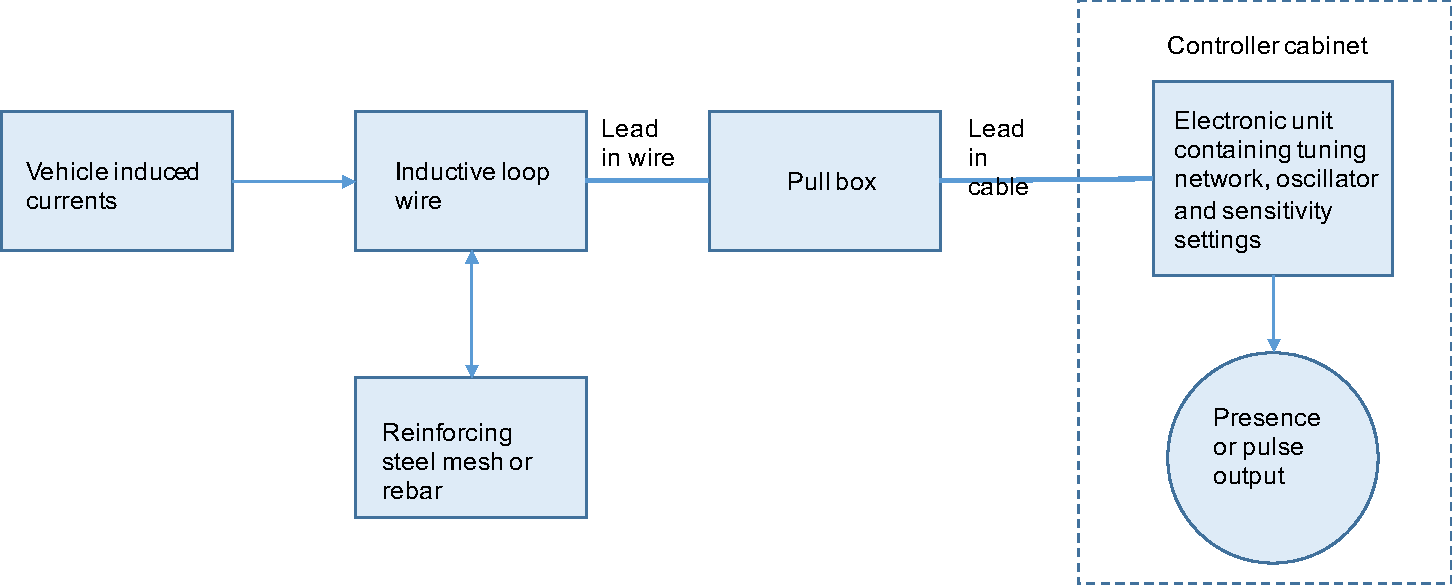
\includegraphics[width=0.7\textwidth,height=0.7\textheight,keepaspectratio]{Figures/loop-detector.pdf}
    \rule{35em}{0.5pt}
  \caption[A vehicle loop detector system]{An inductive loop detector system used for detecting the
  presence or passing of a vehicle. (Source - \textit{Traffic Detector Handbook: Third Edition—Volume I})}
  \label{fig:loopDetector}
\end{figure}

For this study a relatively large data set was used. This data set contains loop detector data collected
at several detection points in and around the Melbourne CBD. This dataset is a homogeneous set of
1084 road sections. A homogeneous section of the road is where the traffic flow normally remains unchanged
during the measured time period. The data was aggregated to a 15 minutes interval over a period
from 01/01/2007 to 25/07/2012, making a total 195168 observations.

\subsection{Measurement errors}
There are various factors that contribute to the measurement errors in traffic volume data. This can
at the vehicle loop detection system or at the traffic control centre. The electronic unit that
detects the change in frequency may not always be accurate leading to a false or missing reading.
We present the data caused by errors in two groups - missing data and false or unreliable data.

\subsubsection{Missing data}
Missing data occurs often in the case where either the loop detection system or the computer system
at the control centre goes down. The missing period could vary between minutes to days depending on
the detection and resolution of the fault. Secondly the data could be missing for a certain location
or a set of locations.


As the data we acquired has zero value for missing data, it is difficult to say if that a zero value
is a result of missing data due to fault or a valid actual measurement. However we can aggregate the
data at a daily level, which then gives us a more better view of the missing data phenomena. Figure
\ref{fig:missing-days-count} shows the number of days for which no measurement was recorded for each
of the 1084 locations.

\begin{figure}[htbp]
  \centering
    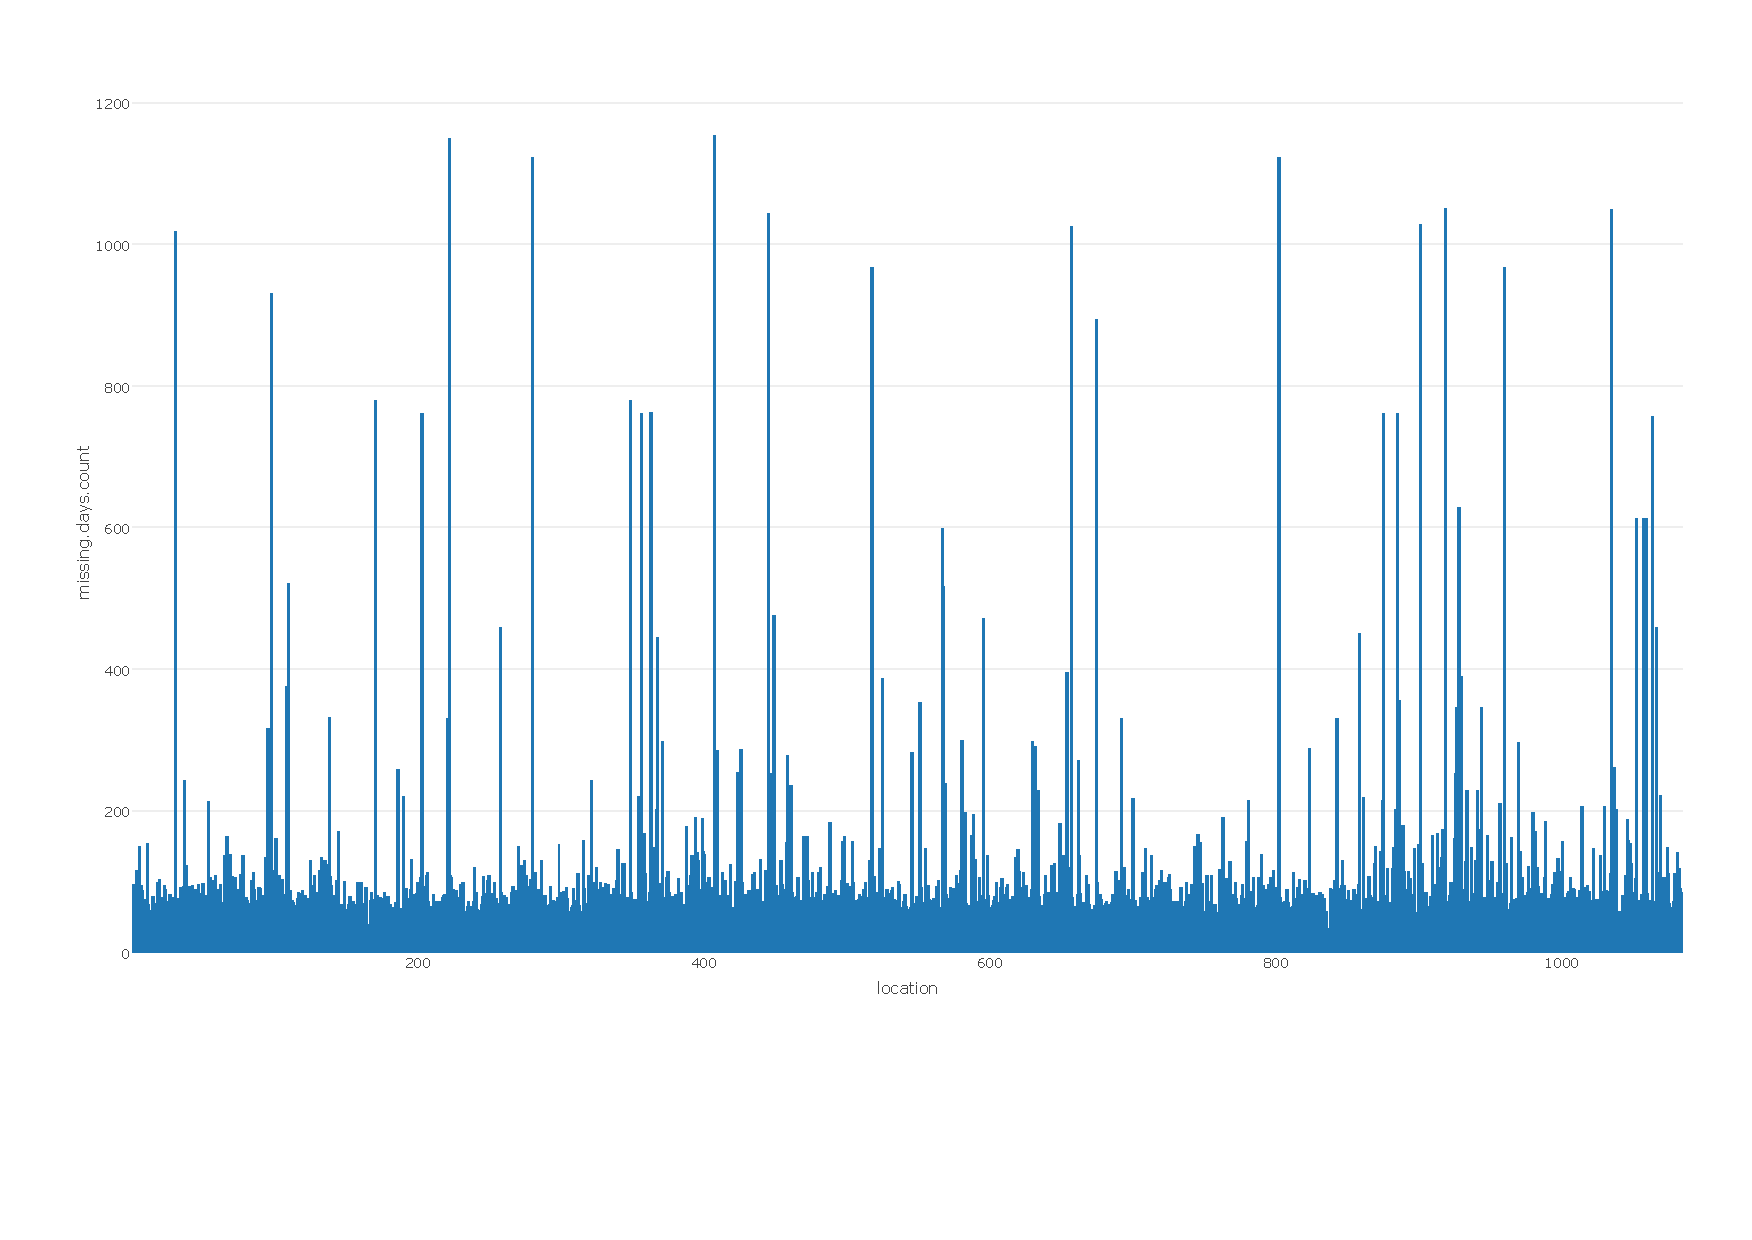
\includegraphics[width=\textwidth,height=\textheight,keepaspectratio]{Plots/missing-days-count.pdf}
    \rule{35em}{0.5pt}
  \caption[Missing data]{Missing data - number of days when no measurement was recorded at each of
  the 1084 locations in our data. The locations are shown as index numbers.}
  \label{fig:missing-days-count}
\end{figure}

We can see the number of missing data it is quite significant and it can largely affect the model for
short term traffic prediction. There are several imputation strategies that are usually used in practice
to deal with missing data in traffic data. One of the methods is known as historical imputation. In this
method previously collected data at similar time interval at the same location is used to fill in the missing
value. The distance in time is often selected as minimum as possible. A variation of this is another
simple approach that takes an average of past few recorded observations and uses that to fill in
the missing data. A second method that is used is spline/linear regression regression that interpolates
the missing value from neighbourhood data points.

\subsubsection{Unreliable data}
Unreliable data is observed when the measurements recorded by the loop detectors show unreasonably
large deviations. This is due to some fault in the loop detector system. These are obvious to the
naked eyes when looking at the plot of the measurements but hard to detect automatically. Such errors
are usually detected during preprocessing by setting a maximum value that a measurement can have. The
maximum value can be obtained using the frequency distributions of the measurements.

\section{Analysis of the traffic volume data}

% location lat-lng (start -37.8099,144.9913, end
In this section, we present a moderate analysis on the traffic volume data mentioned earlier in
previous section. An in depth analysis on traffic flow, covering all the factors that influence the
short and long term variations, extends beyond the scope of the work. For the purpose of our analysis
we chose the location with the least number of missing data. This location is a road section(HF No.
16913) on Victoria street between Hoddle street and Church street, which is located on the north-east
of Melbourne CBD. This is shown in the figure \ref{fig:ExperimentRegion} annotated in red. The region
in  blue is the neighbourhood of this section road, which is used to find spatial correlations. This
region is further used for experiments and evaluation of various traffic prediction models, presented
in chapter \ref{Chapter5}.

\begin{figure}[htbp]
  \centering
    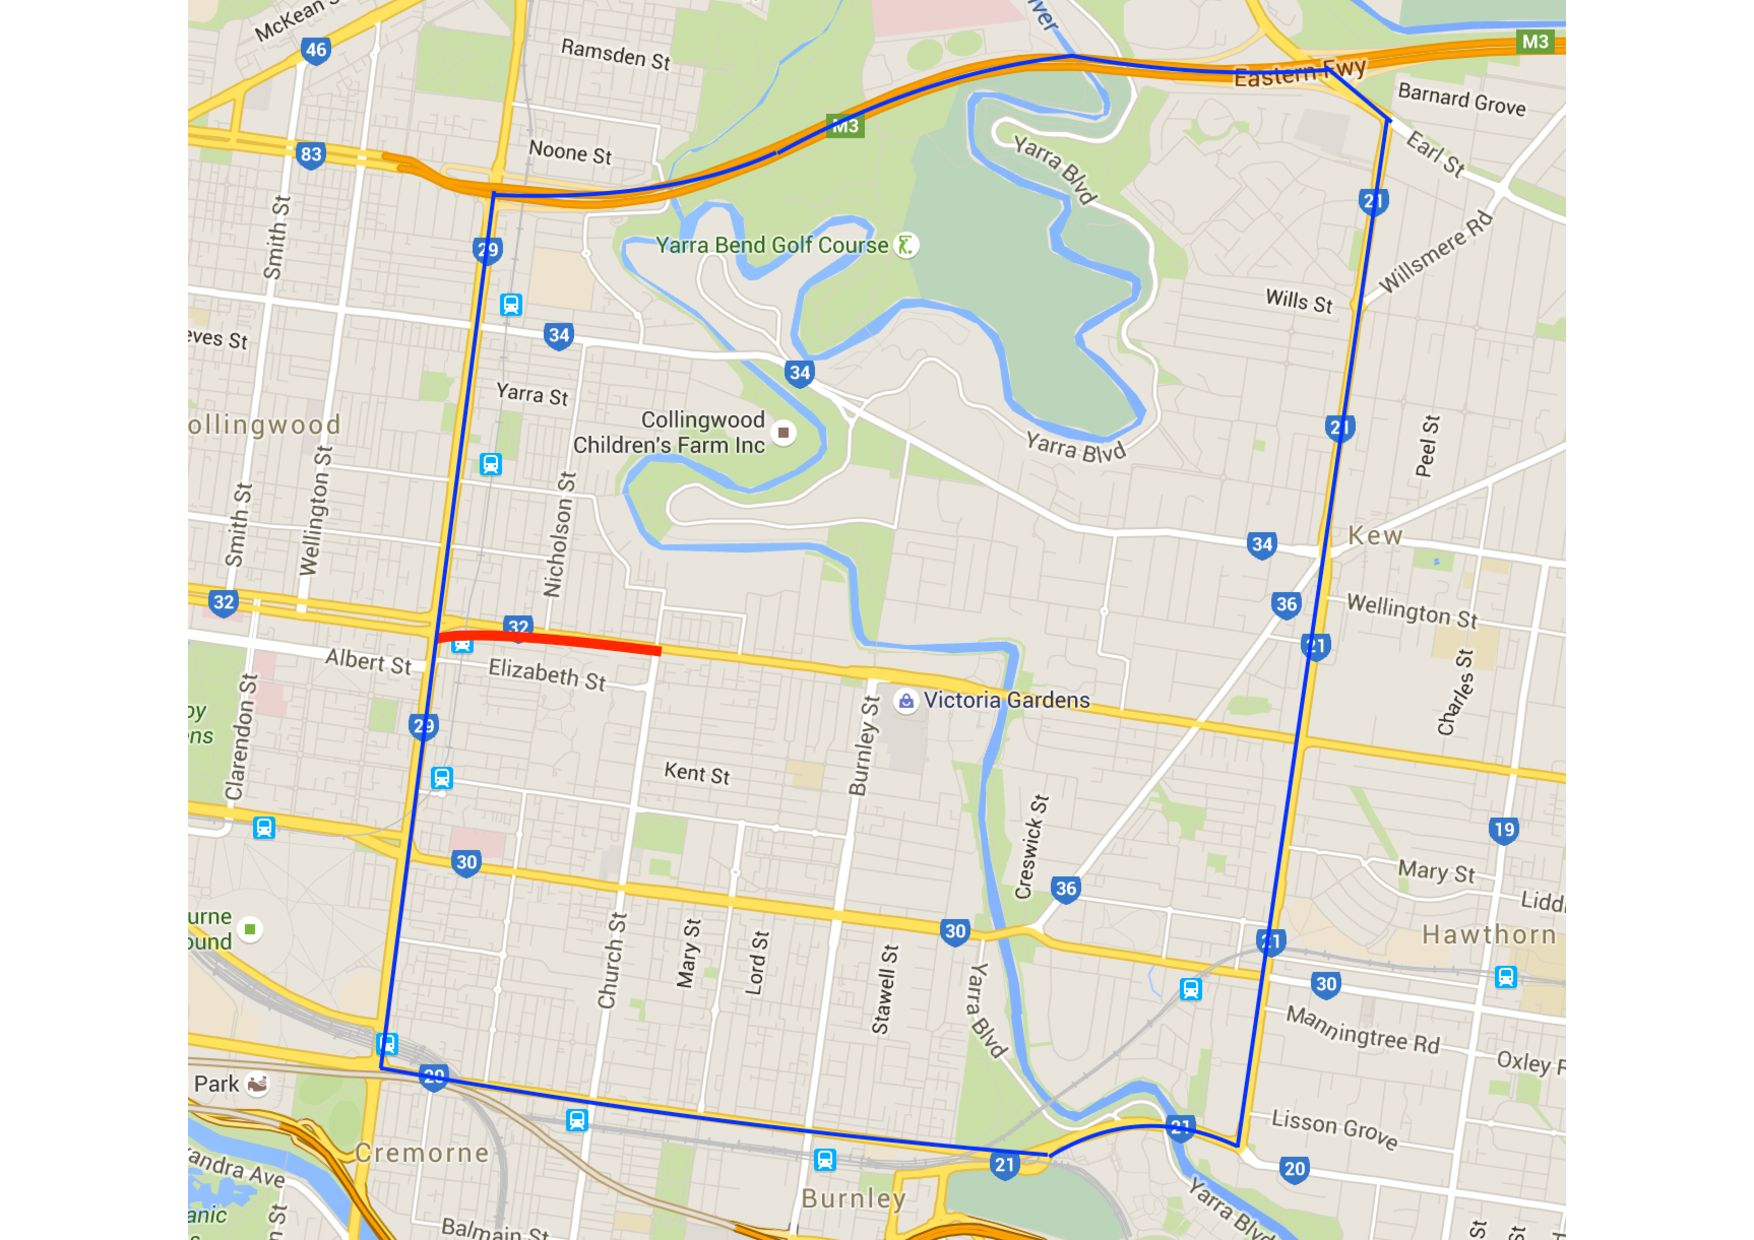
\includegraphics[width=\textwidth]{Figures/experiment-region.pdf}
    \rule{35em}{0.5pt}
  \caption[Experiment traffic region]{The traffic region used in this experiment. The boundary is
   dentoed by the red line. Source - \textit{Google Maps}}
  \label{fig:ExperimentRegion}
\end{figure}


\subsection{Variations and trends}

\subsubsection{Systematic variations}
Recurrent daily variations in traffic flow data exhibit similar behaviour at a location for
a particular day. These variations are caused by travel demands of day to day activities. In
general, for any particular day we can segment the traffic flow into following components -
peak hours usually one in morning and one afternoon, off-peak hours, evening hours and night hours.
These can be easily examined using simple visualisations. Let us inspect how average traffic volume
changes over time during a day. We first group the volume data into two categories - weekdays and
weekends and present the plots in figure \ref{fig:dailyVariations},

\begin{figure}[htbp]
    \centering
    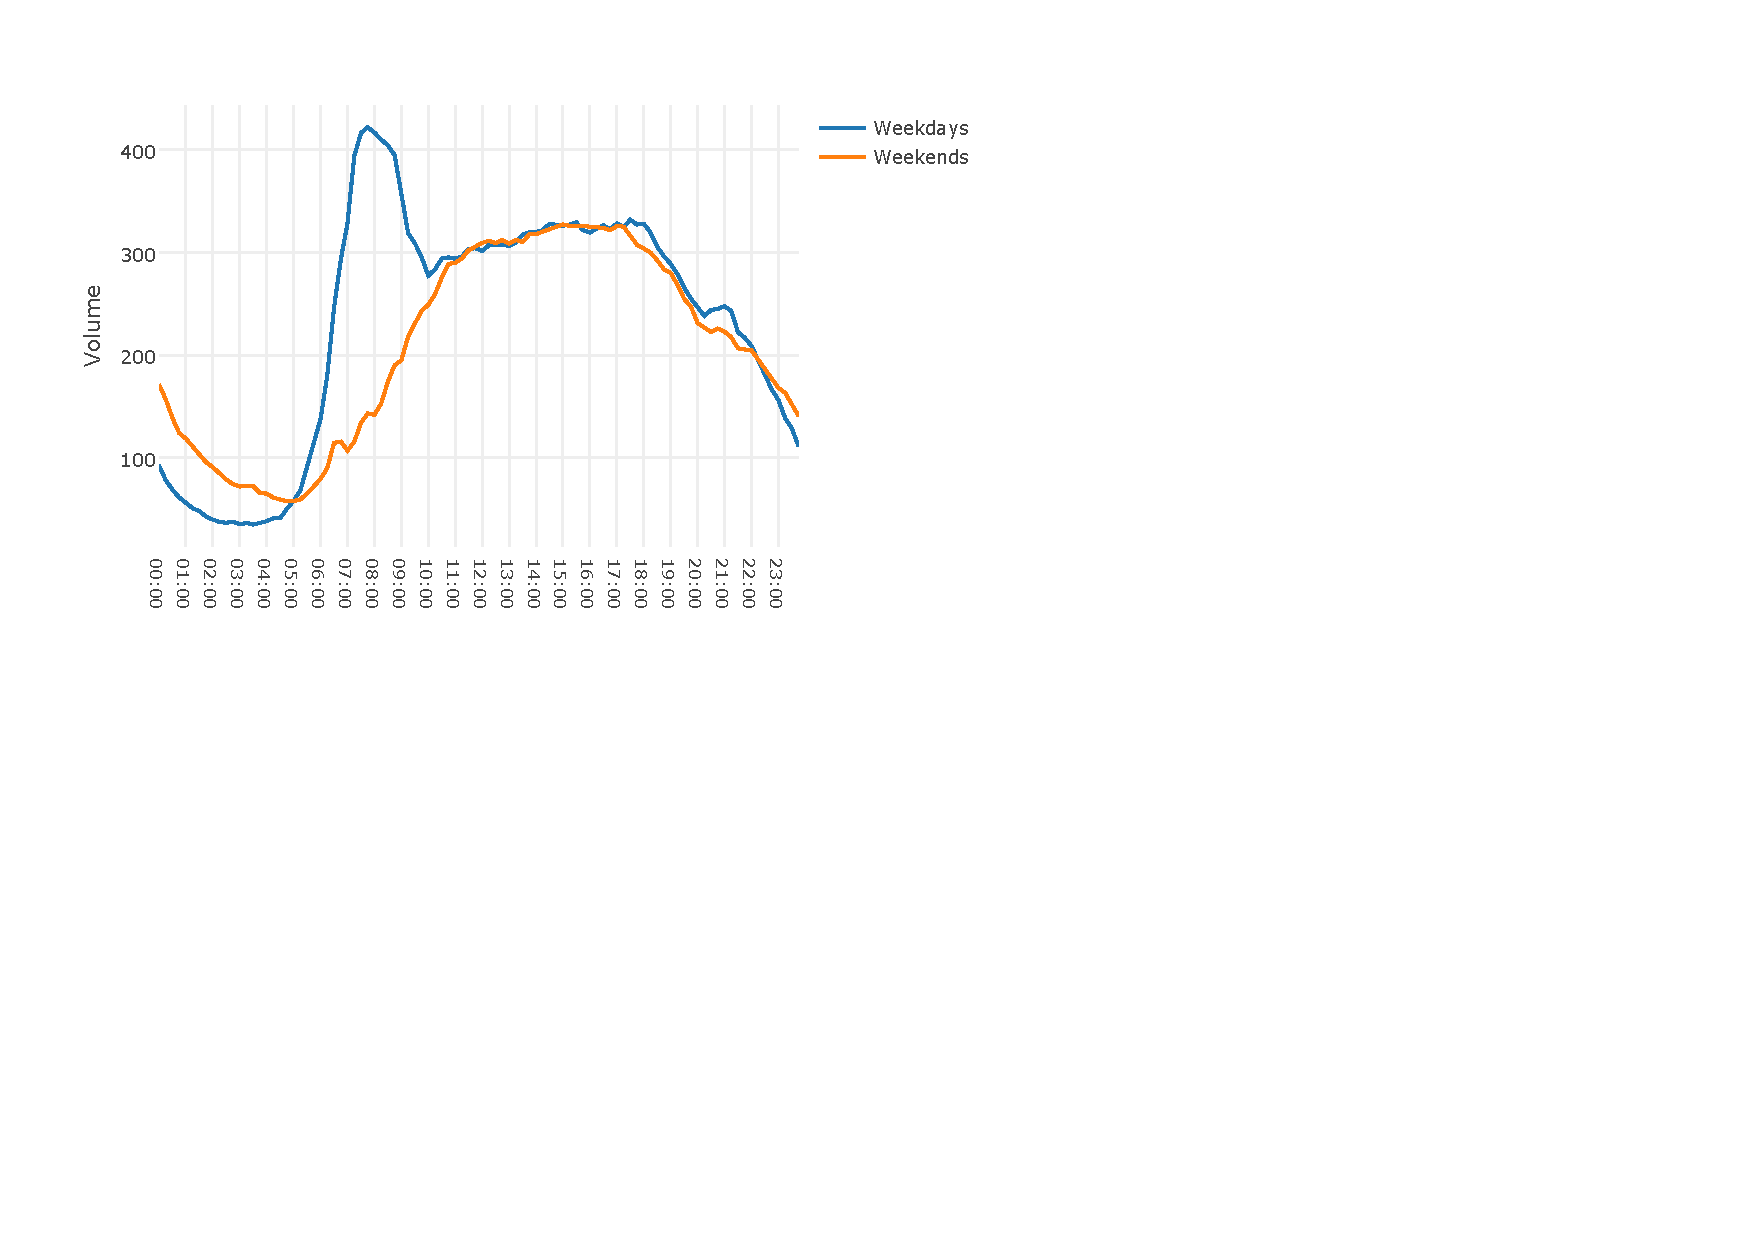
\includegraphics[width=\textwidth]{Plots/average-day.pdf}
    \rule{35em}{0.5pt}
    \label{fig:averageDay}
  \caption[Average traffic flow on weekdays and weekends]{Variations in average traffic flow
  at 15 minutes interval grouped by weekdays and weekends.}
  \label{fig:dailyVariations}
\end{figure}

We can see from the plot that, a significant difference in how traffic flow changes during the
course of a week day and a weekend. On weekdays we can see a steep rise in the traffic flow in the
morning between 7AM and 9AM. Another peak is seen at the evening time between 5PM and 6PM. These
sudden changes in traffic flow are mainly because of the traffic caused by getting to and coming
from work. There is also a steep drop in traffic that starts at 9PM. On weekends the variations do
not have such steep rises and falls, rather the traffic slowly builds up and stays almost stable
throughout the afternoon and then slowly starts to drop. These variation on weekends can mainly be
attributed to personal activities.


However traffic flow on each day of the week is also different. In figure \ref{fig:TypicalDayTraffic},
we plot the daily variations in traffic. From this we can infer the morning peak is highest on
Thursdays, while Mondays have the least of the morning peaks among all weekdays. During afternoon
there is not a large difference in the peak among the days. We can also see on Friday and Saturday
the drop in traffic flow happens much later than the other days and also the drop is less steeper.

\begin{figure}[htbp]
    \centering
    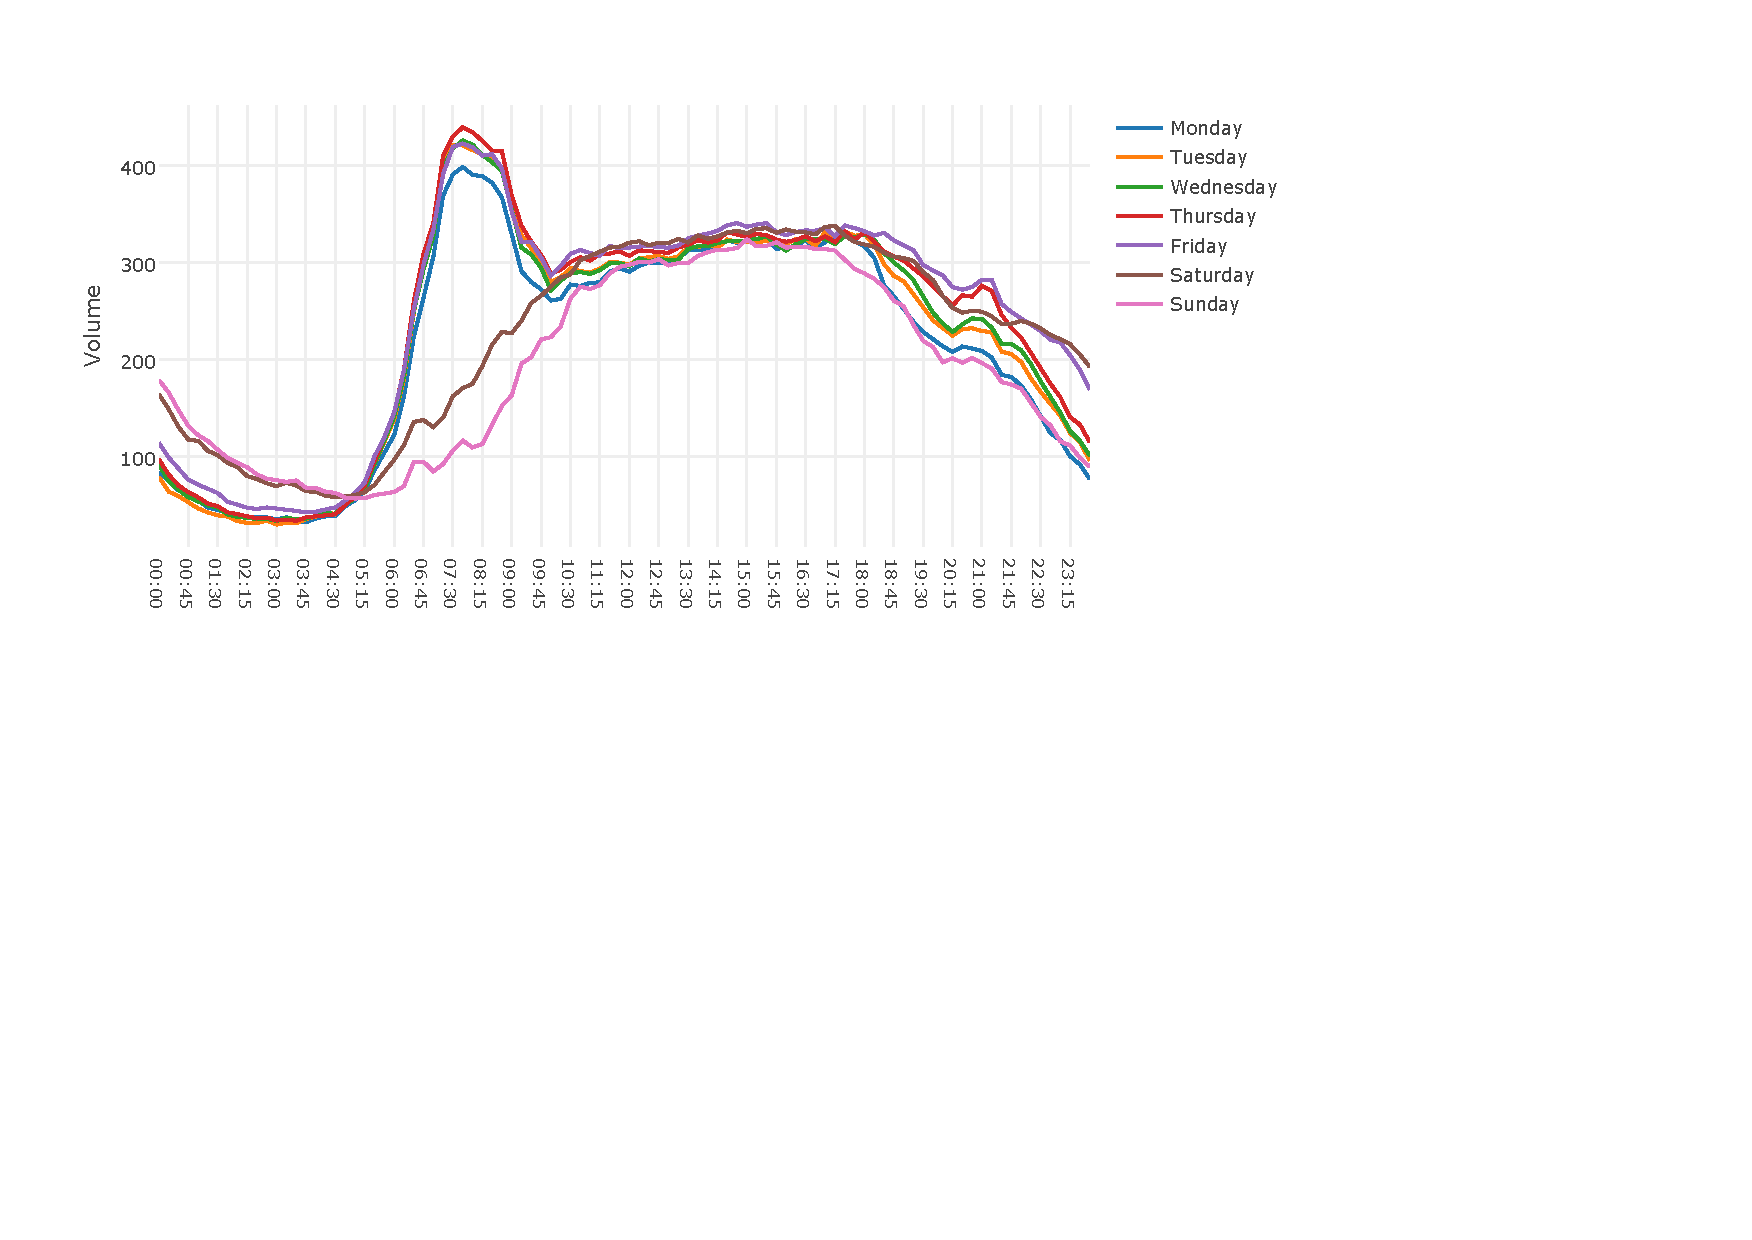
\includegraphics[width=\textwidth]{Plots/average-group-day.pdf}
    \rule{35em}{0.5pt}
    \label{fig:averageGroupByDay}
  \caption[Average traffic flow grouped by day of the week]{Daily variations in traffic flow, the
   above plot shows average 15 minute traffic flow grouped by day of the week}
  \label{fig:TypicalDayTraffic}
\end{figure}


Similarly during the course of a month, traffic flow on an average day can be different for different
weeks. Again to observe these variations we plot the average traffic volume for four weeks
of the month of January, April, July and October. This is shown in figure
\ref{fig:MonthlyVariations}. From this we can not tell any consistent difference in average traffic
flow on each of these four weeks.

\begin{figure}[h]
    \centering
    \subfloat[January][January]{
    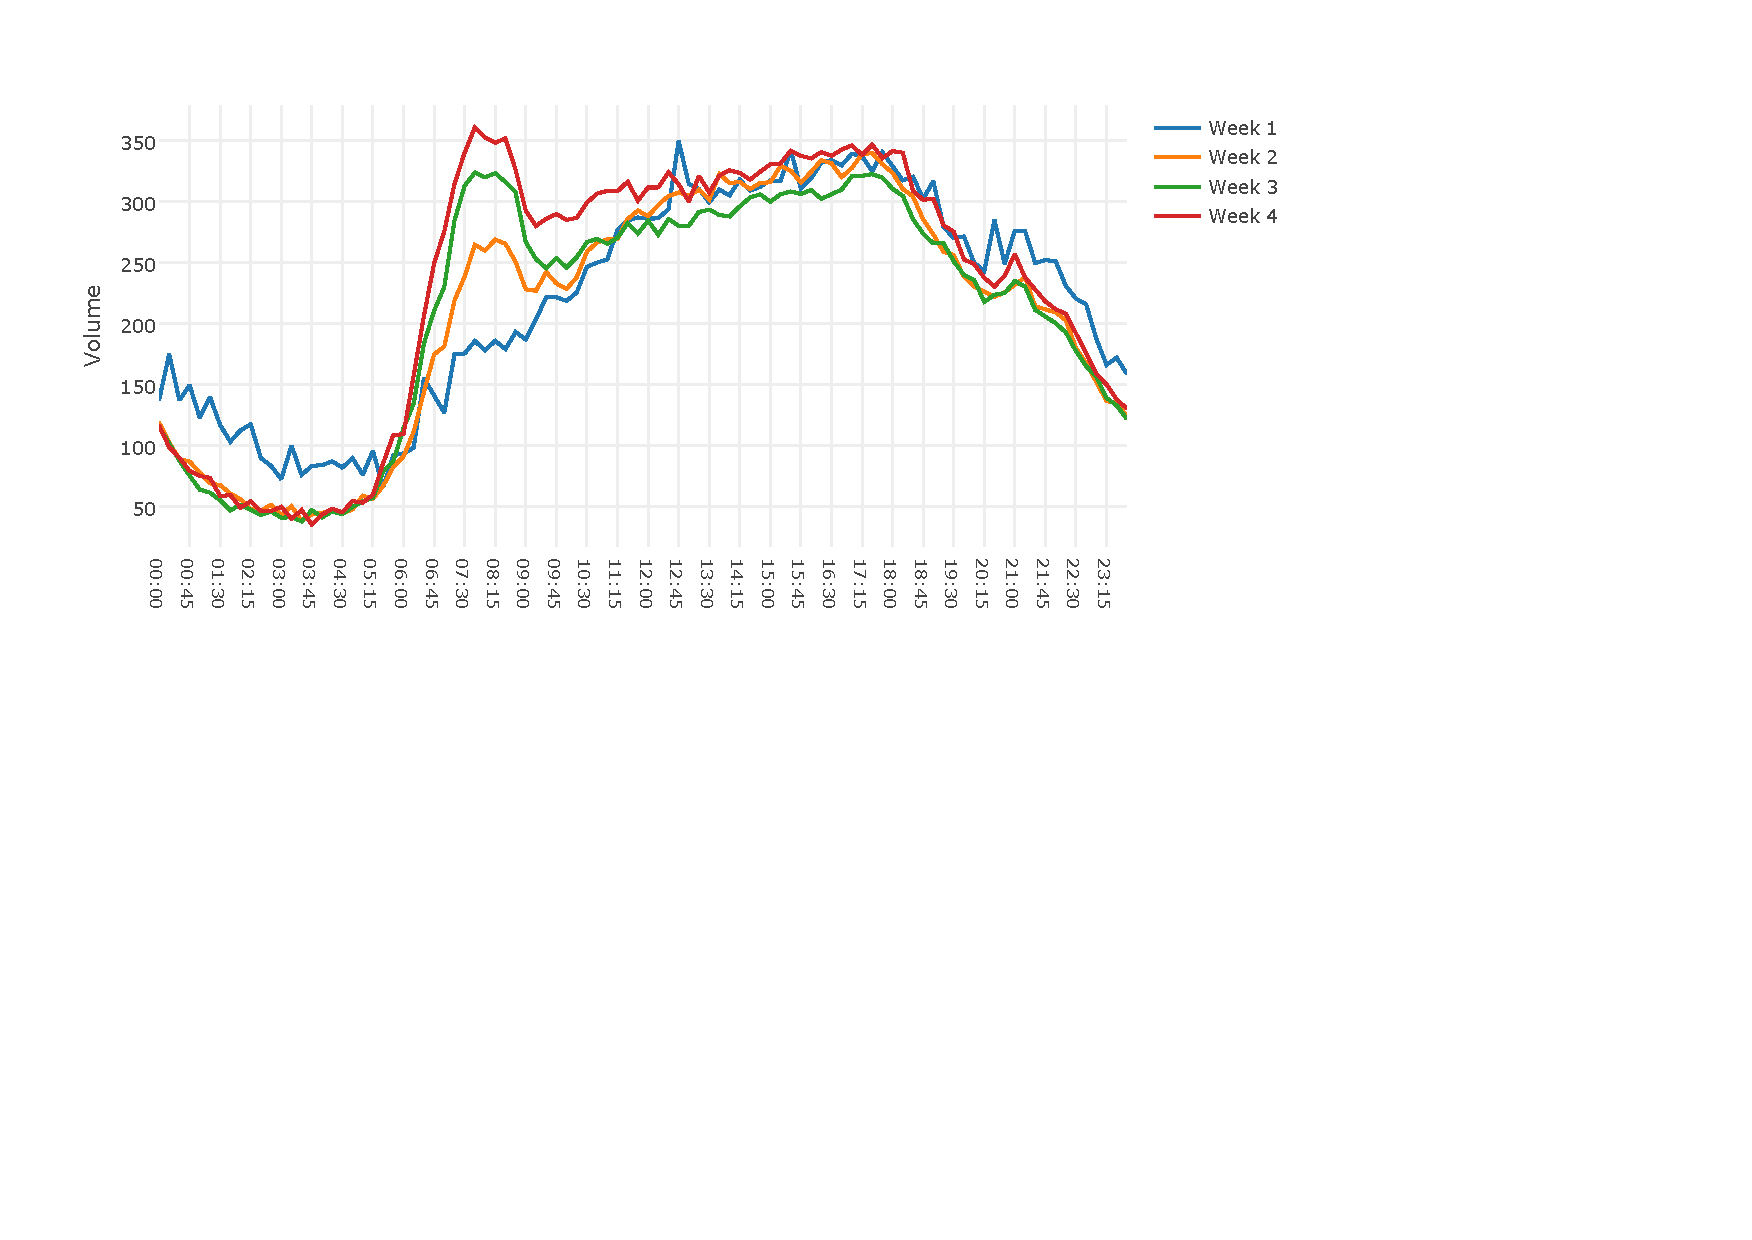
\includegraphics[width=0.4\textwidth]{Plots/weeks-jan.pdf}
    \label{fig:WeeksJanuary}}
    \qquad
    \subfloat[April][April]{
    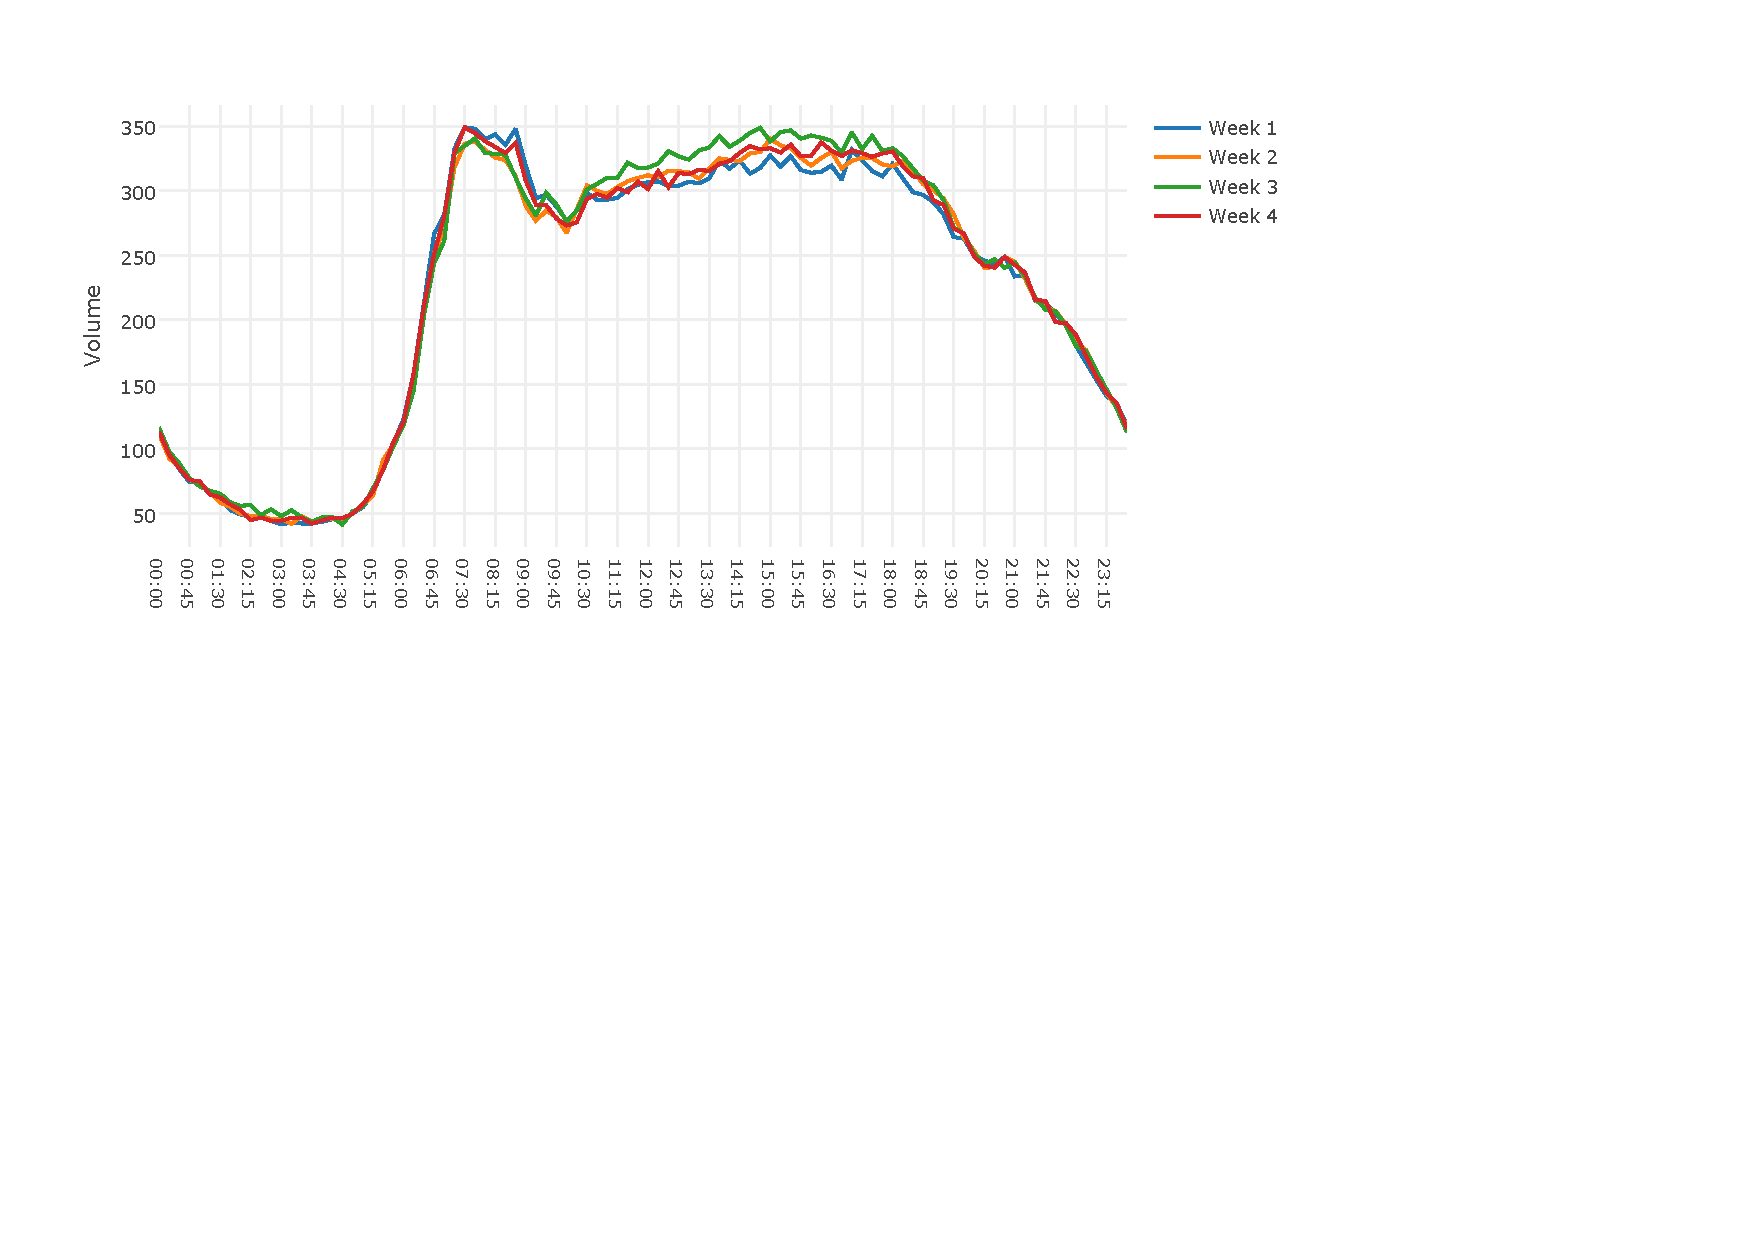
\includegraphics[width=0.4\textwidth]{Plots/weeks-apr.pdf}
    \label{fig:WeeksApril}}

    \subfloat[July][July]{
    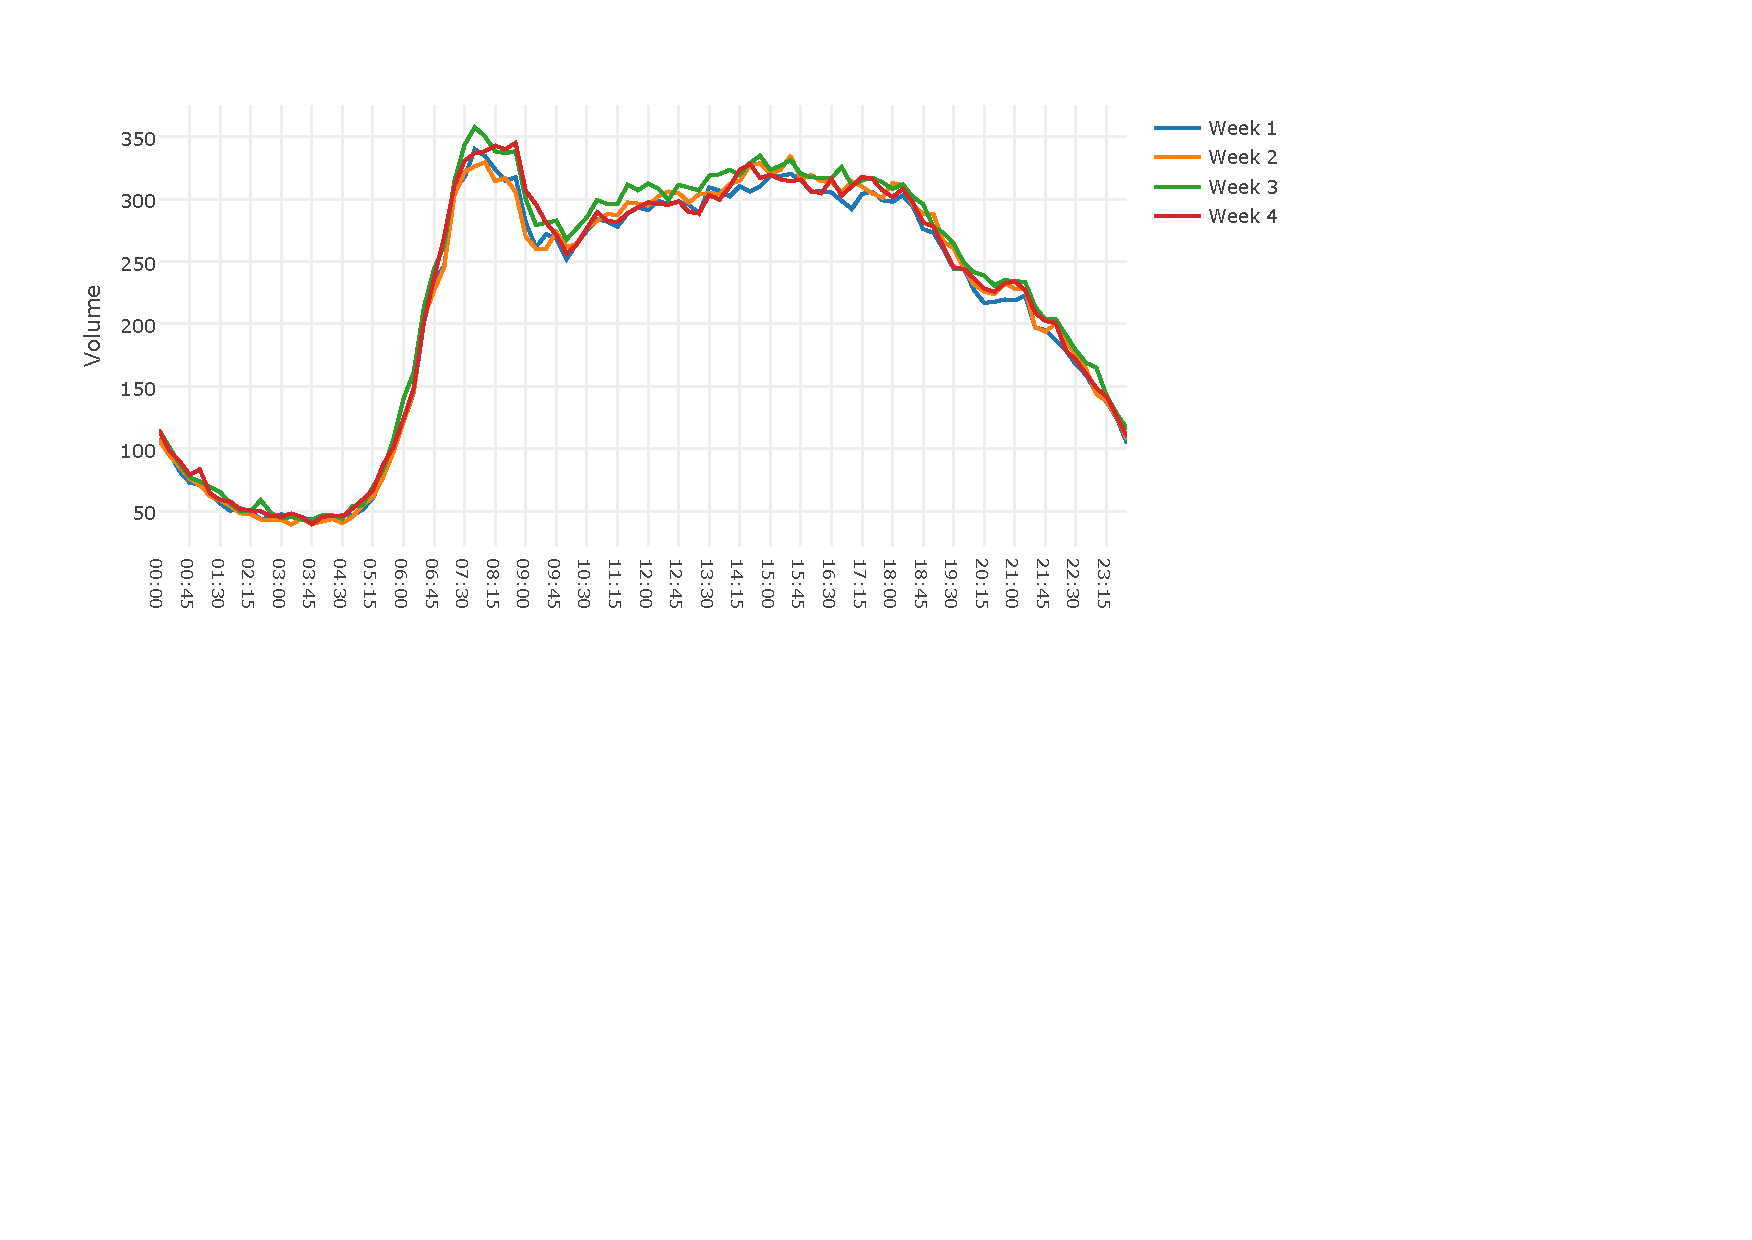
\includegraphics[width=0.4\textwidth]{Plots/weeks-july.pdf}
    \label{fig:WeeksJuly}}
    \qquad
    \subfloat[October][October]{
    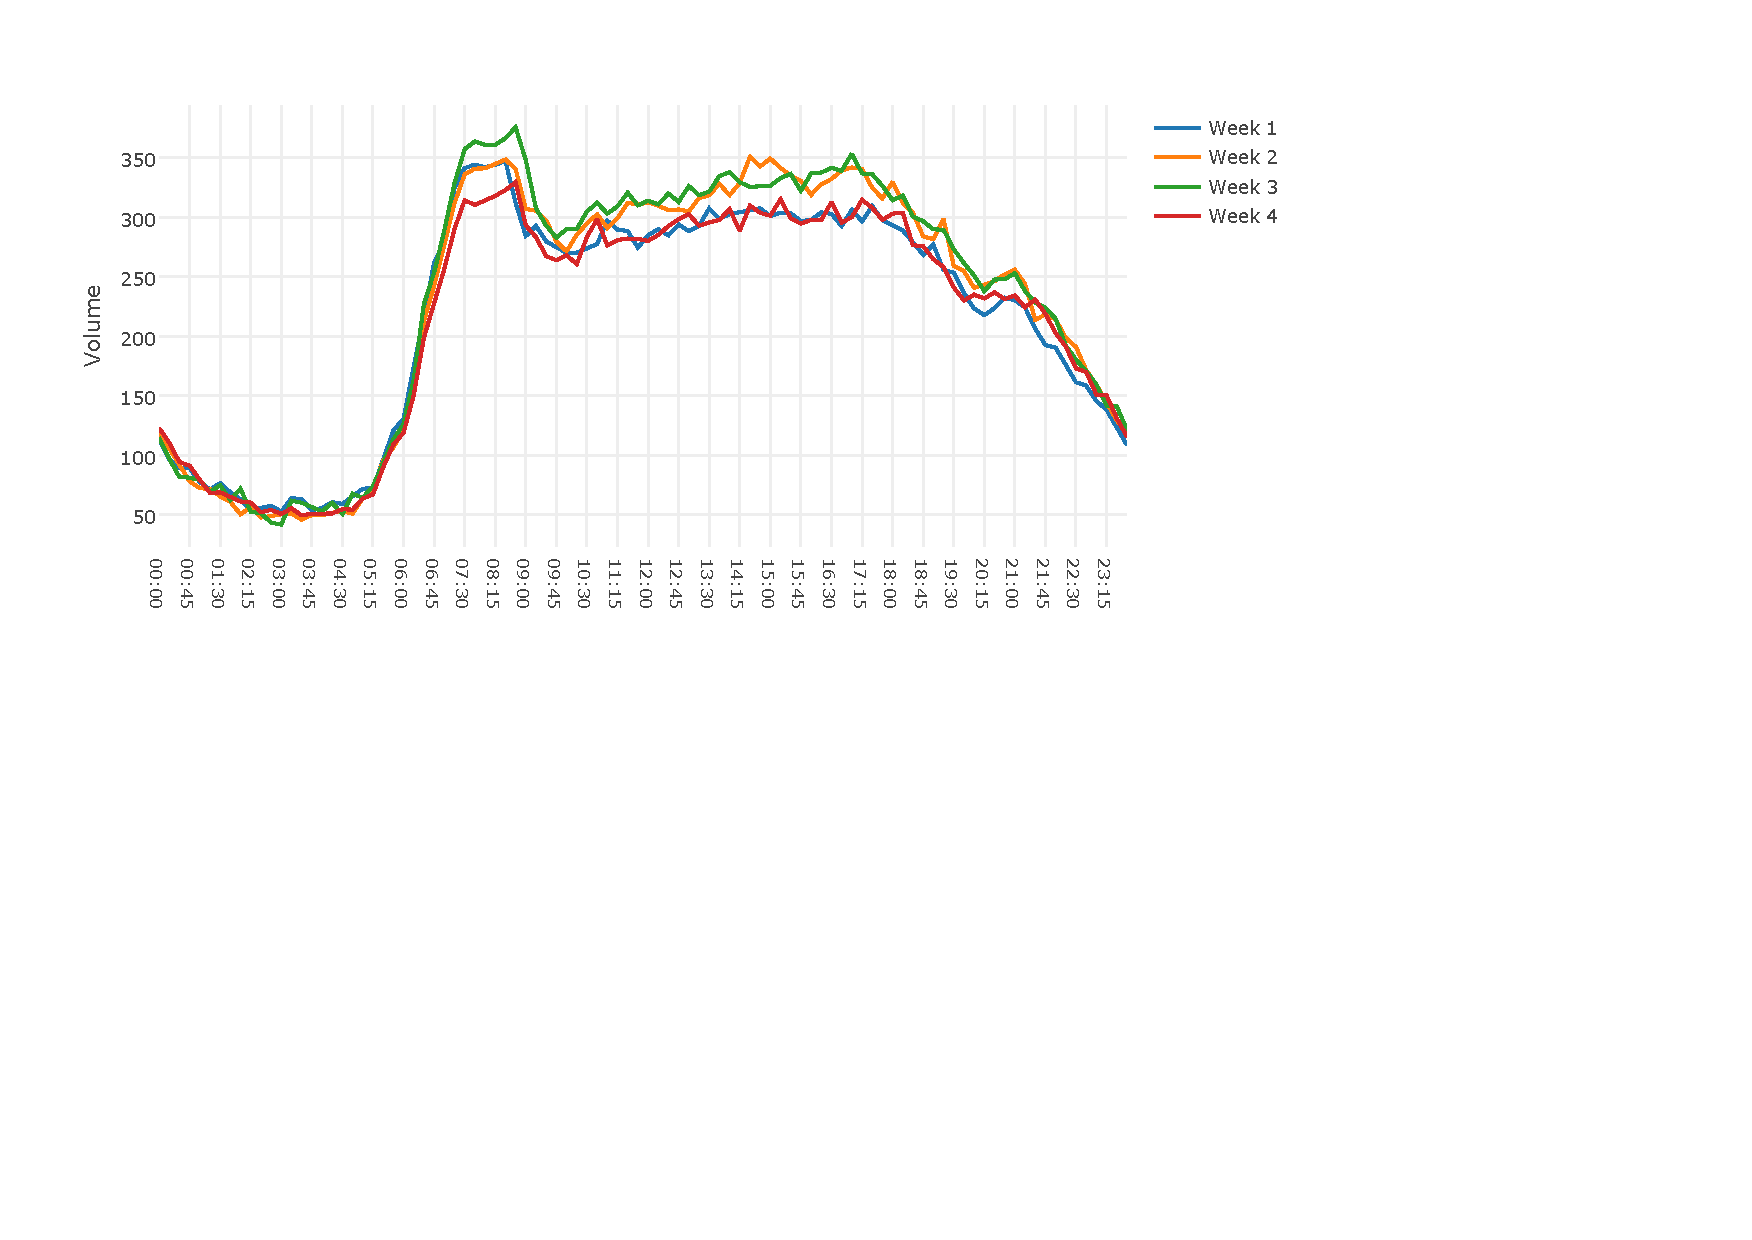
\includegraphics[width=0.4\textwidth]{Plots/weeks-oct.pdf}
    \label{fig:WeeksOctober}}

  \caption[Average traffic flow during a day grouped by weeks]{Average traffic flow during a day in
  a month grouped by weeks. We only show three months here. The plot shows average 15 minute traffic
  flow during the months of January, April and July.}
  \label{fig:WeeklyVariations}
\end{figure}

Finally to find out the changes in traffic flow on an average day of different months of a calendar
year. We can see that the morning peak is lowest in the month of December. The overall traffic
is lower in the months of June and December than the other months.

\begin{figure}[h]
    \centering
    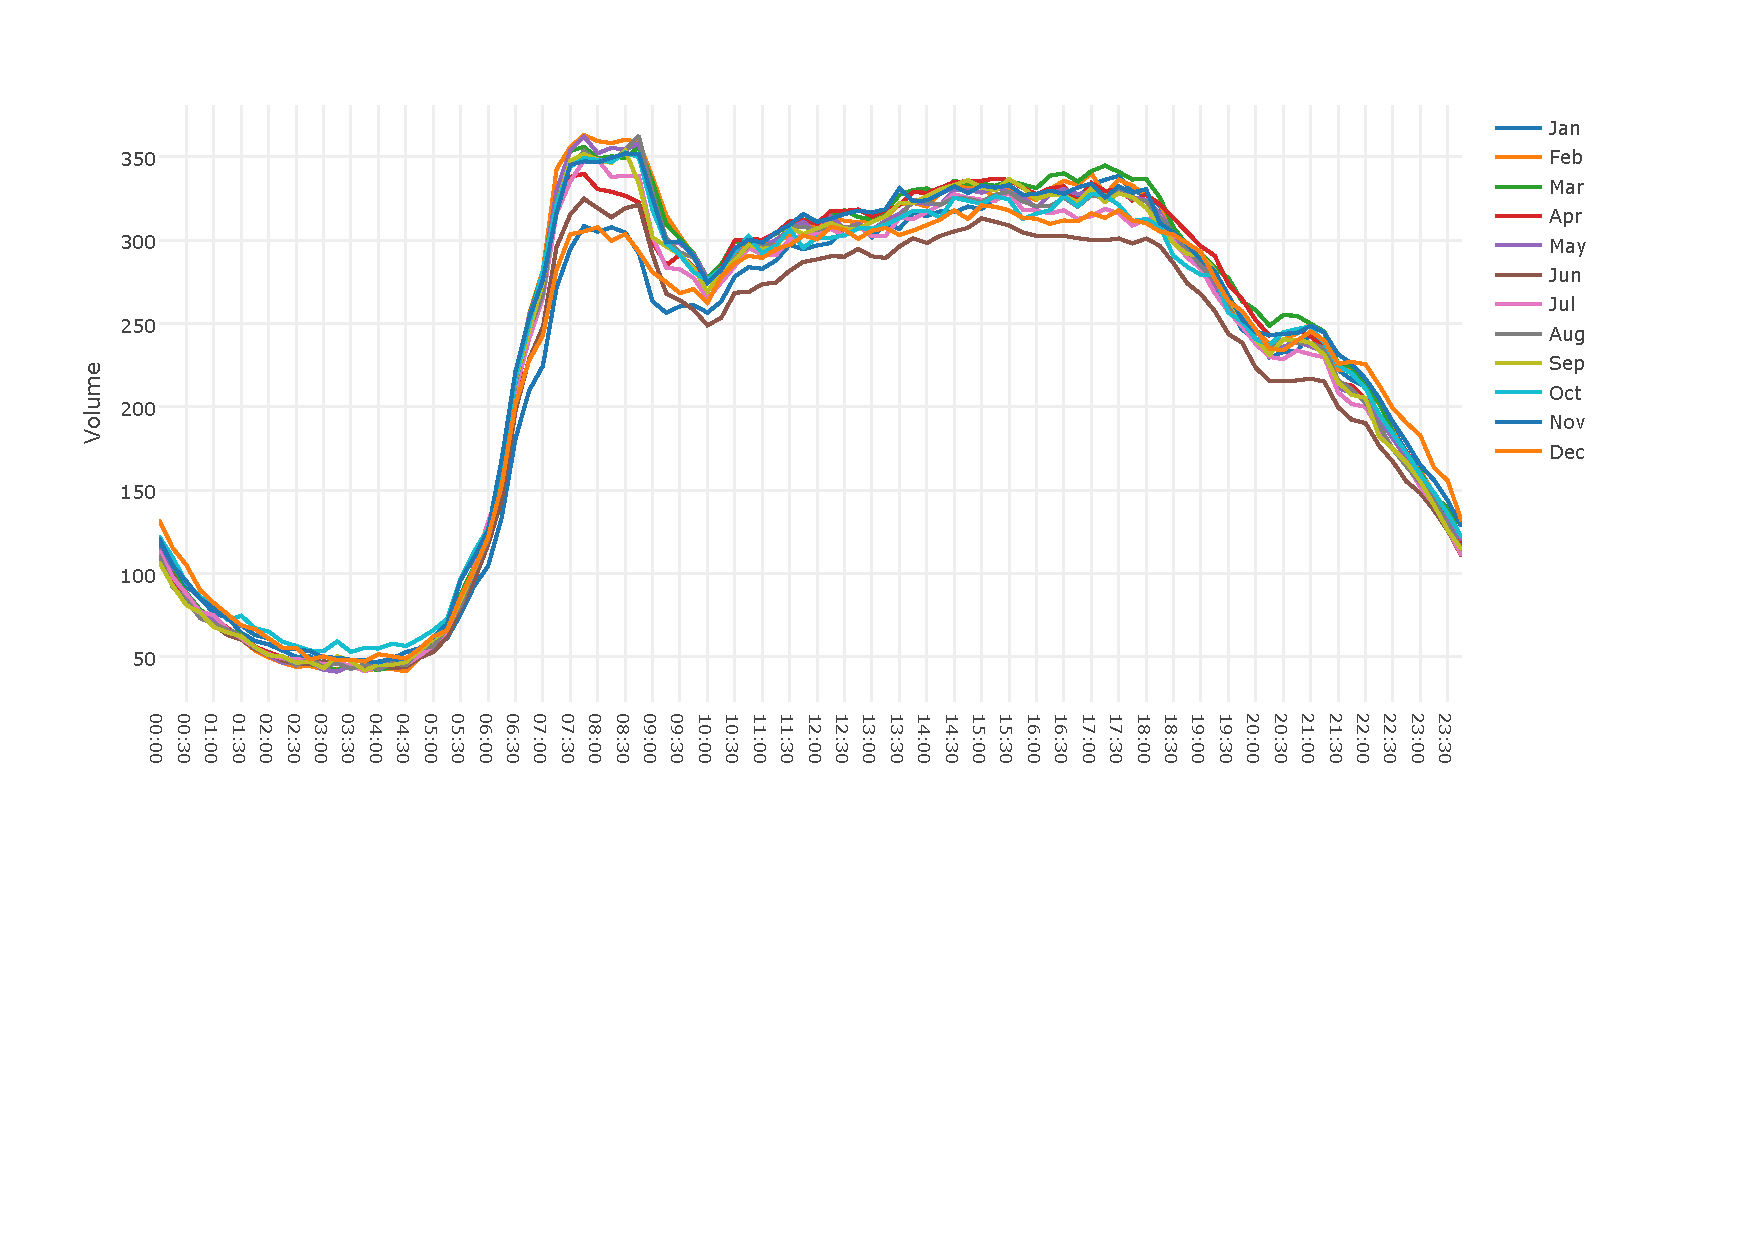
\includegraphics[width=\textwidth,height=\textheight,keepaspectratio]{Plots/variation-months.pdf}
    \rule{35em}{0.5pt}
  \caption[Average traffic flow during a day grouped by months]{Average traffic flow during a day
  grouped by months.}
  \label{fig:MonthlyVariations}
\end{figure}


\subsubsection{Outliers}
Outliers in traffic variations are caused by public events or non-recurrent events such as accidents,
road work etc.  In fig \ref{fig:Holidays}, we plot the traffic flow on public holidays. For comparison
purpose we divided this into five groups based on the day of the week, that is from Monday to Friday.
In each plot we also show the average traffic flow. From these plots we can see different behaviours
in changes in traffic flow on different public holidays. On Easter Monday, Labour day,
Melbourne Cup Day and ANZAC day there is a higher road traffic flow than the average, while on the
rest of the public holidays the flow is significantly lower than the average. So the effect of
public holidays on traffic flow is not obvious and does not follow a consistent pattern.

\begin{figure}[h]
    \centering
    \subfloat[Monday][Monday Holidays]{
    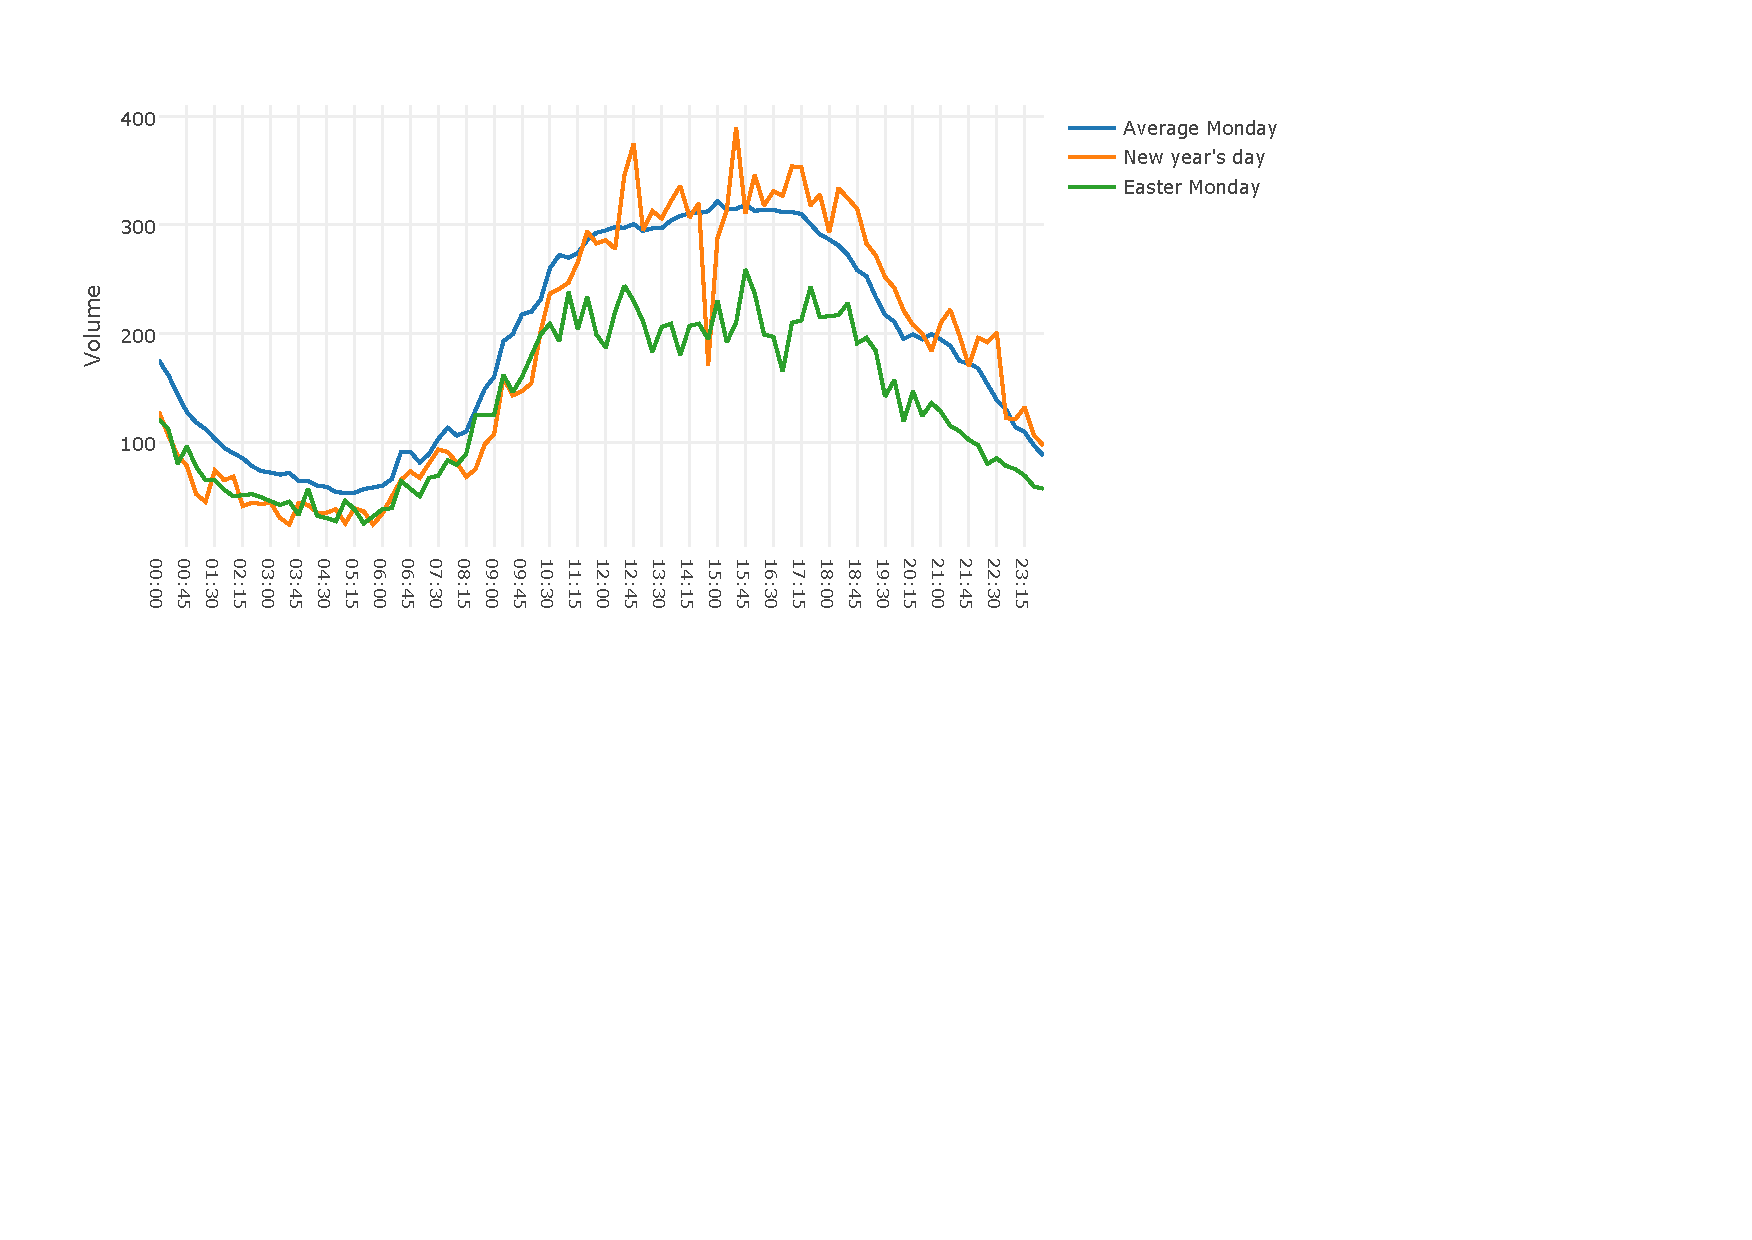
\includegraphics[width=0.4\textwidth]{Plots/holiday-mondays.pdf}
    \label{fig:HolidayMondays}}
    \qquad
    \subfloat[Tuesdays][Tuesday Holidays]{
    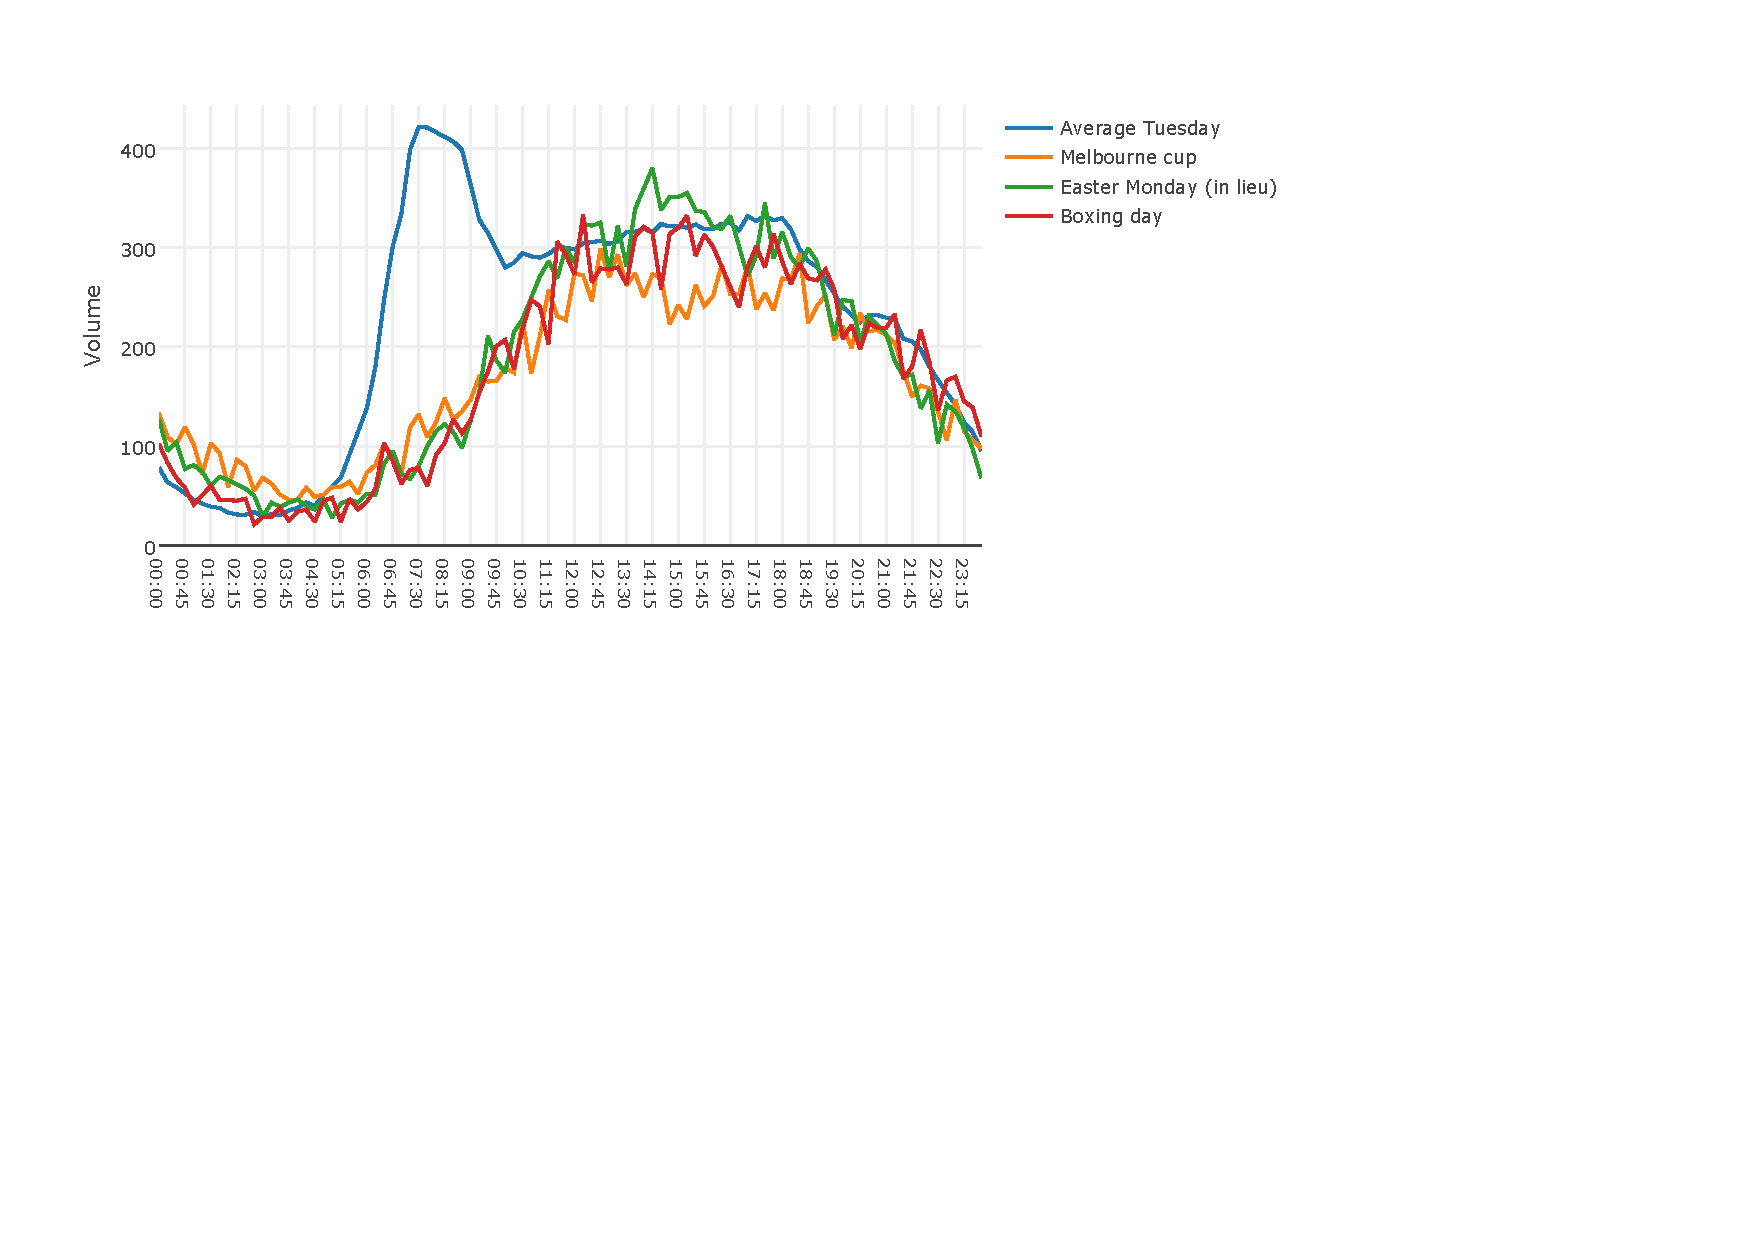
\includegraphics[width=0.4\textwidth]{Plots/holiday-tuesdays.pdf}
    \label{fig:HolidayTuesdays}}

    \subfloat[Wednesdays][Wednesday Holidays]{
    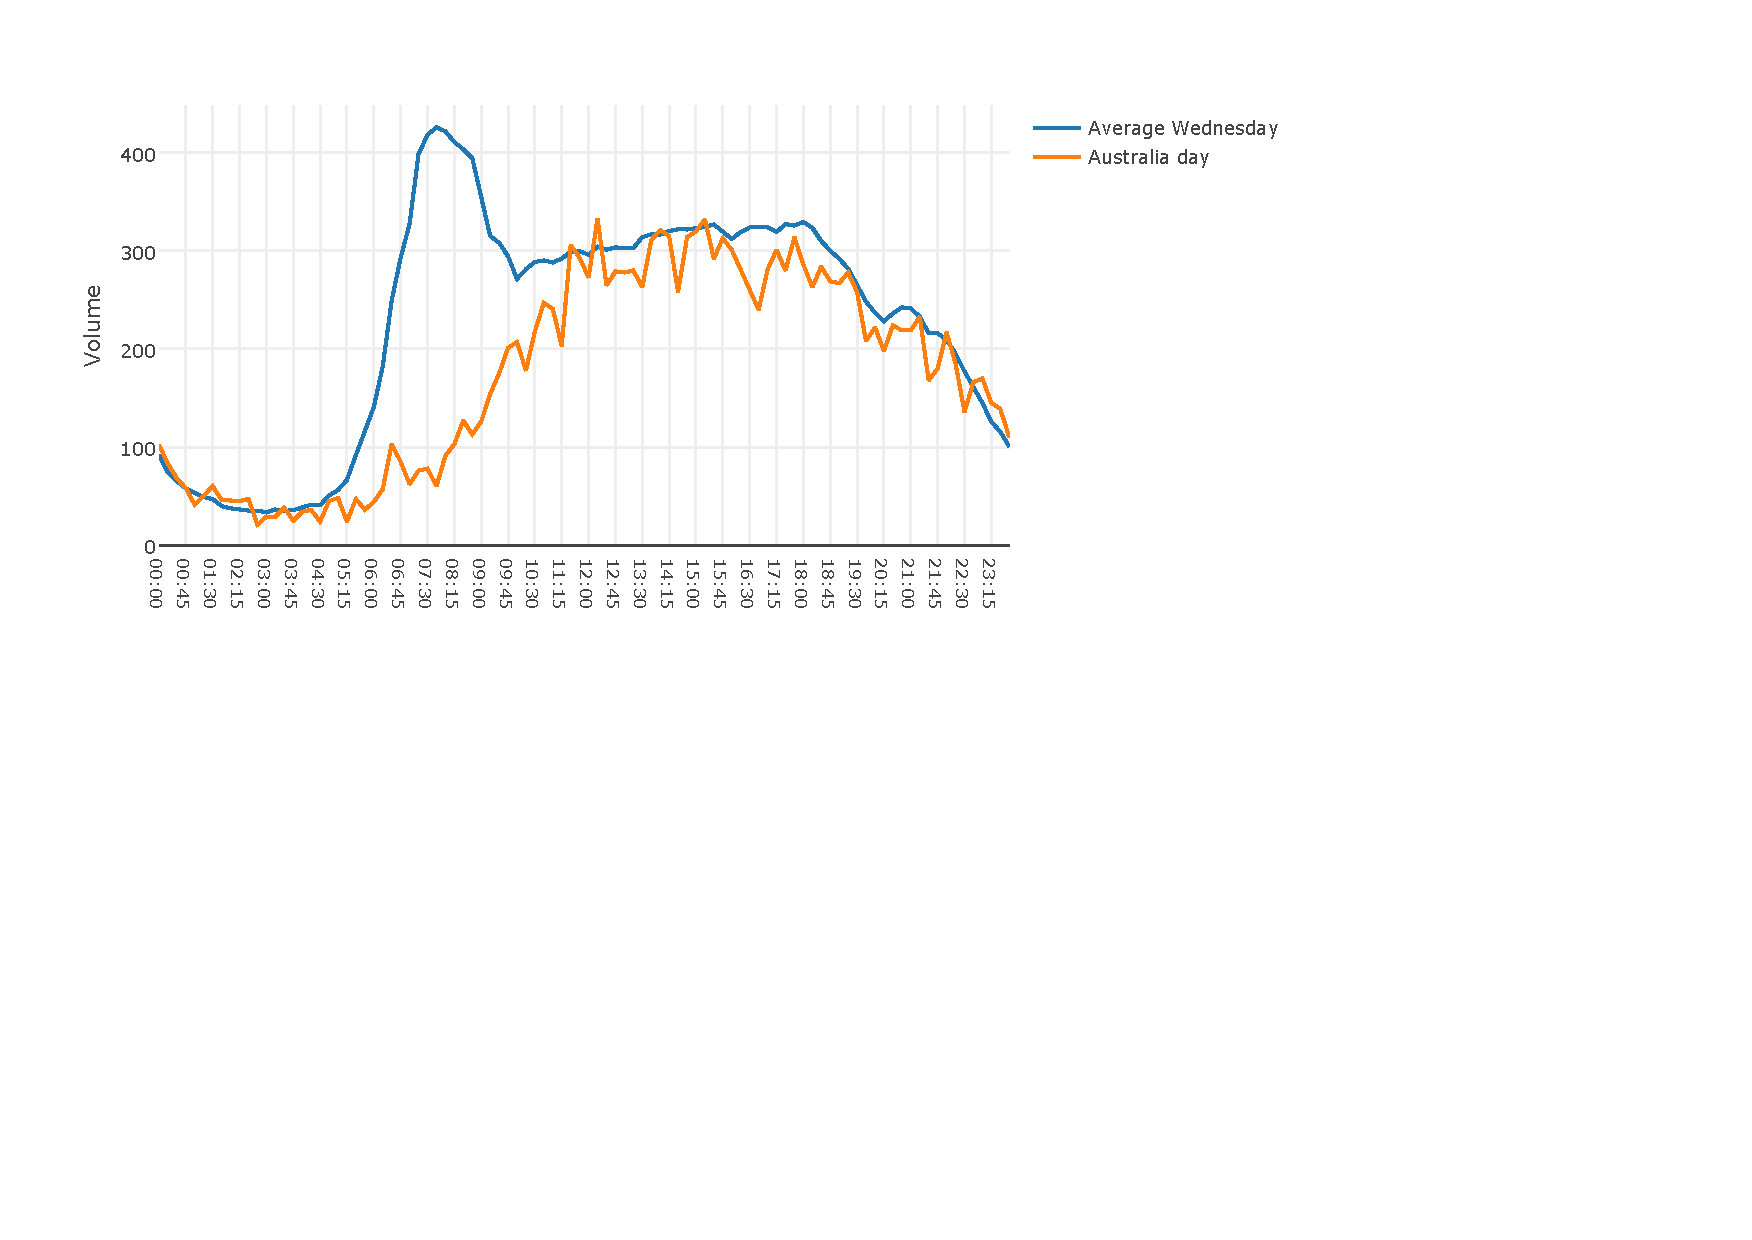
\includegraphics[width=0.4\textwidth]{Plots/holiday-wednesdays.pdf}
    \label{fig:HolidayWednesdays}}
    \qquad
    \subfloat[Thursdays][Thursday Holidays]{
    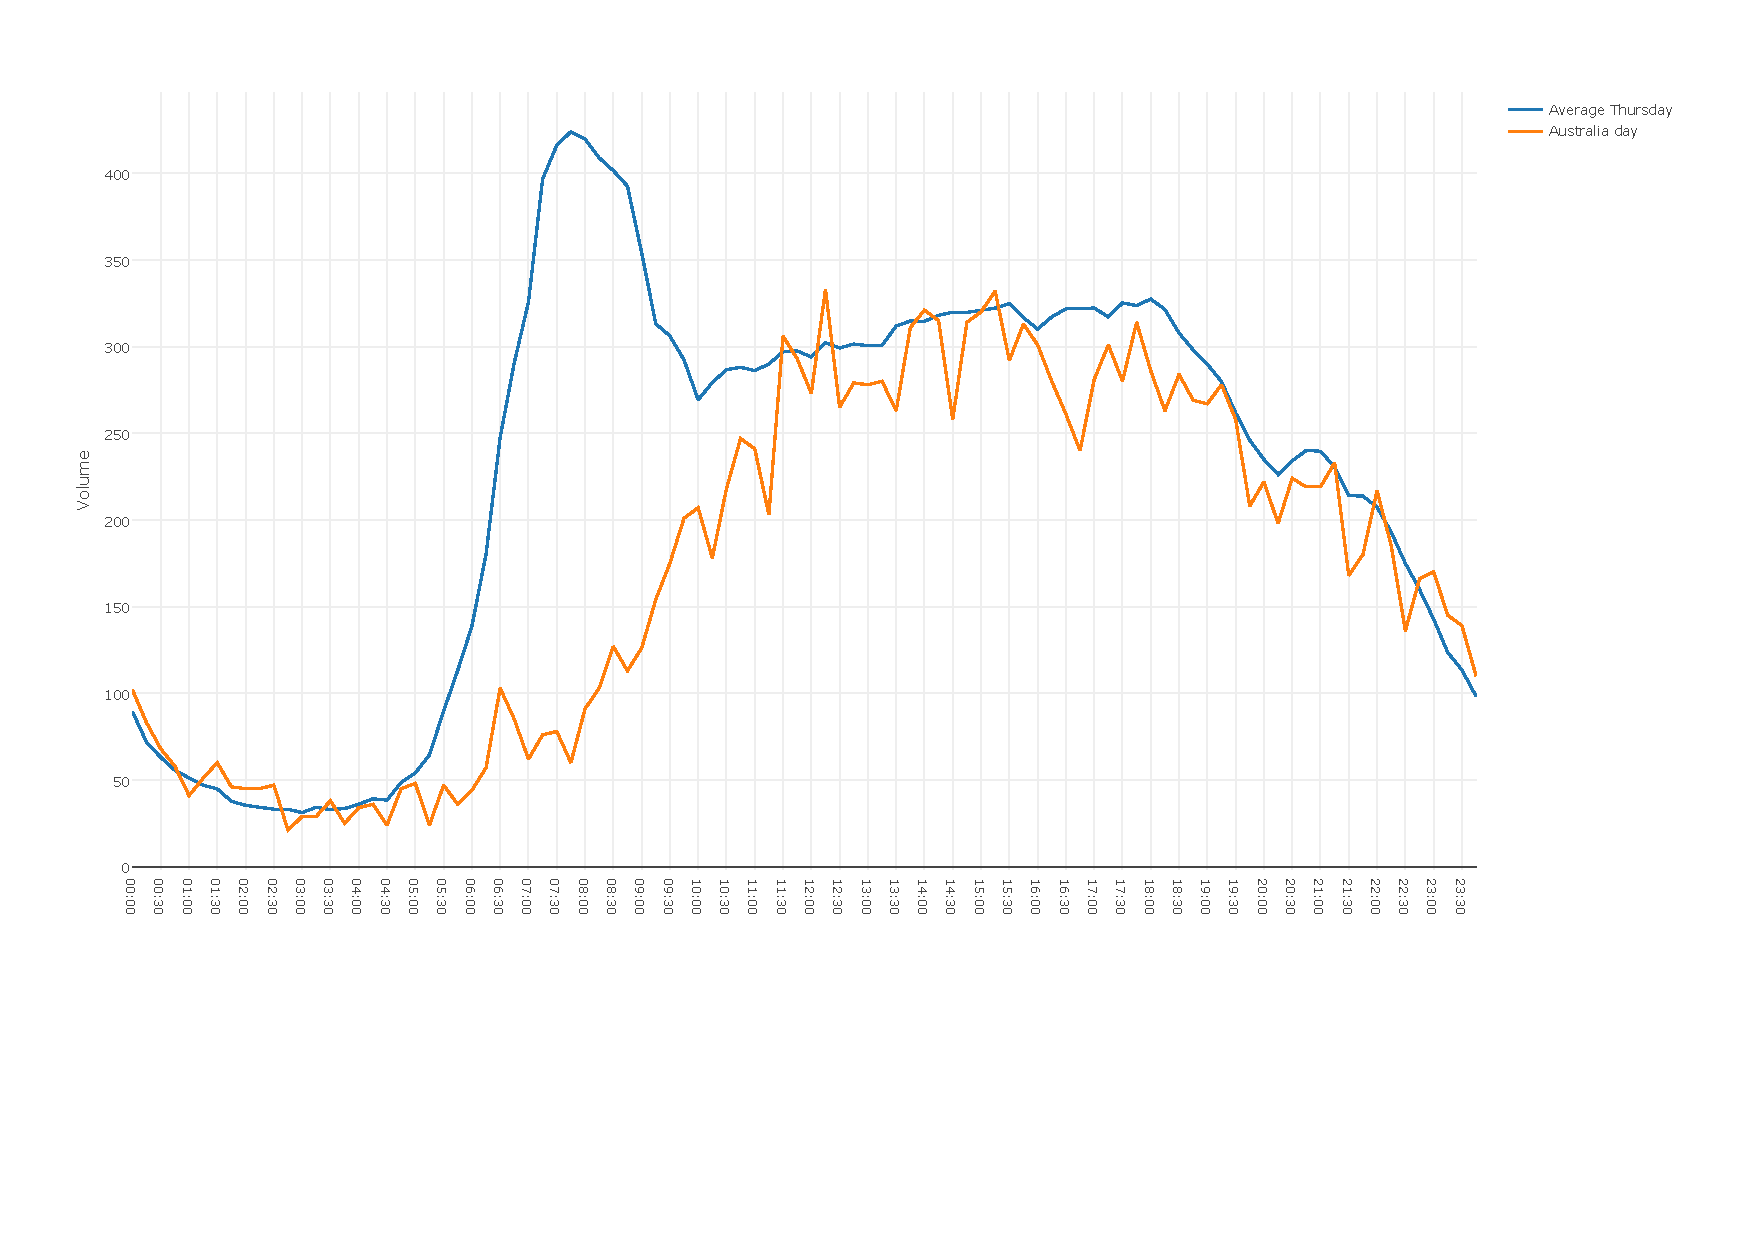
\includegraphics[width=0.4\textwidth]{Plots/holiday-thursdays.pdf}
    \label{fig:HolidayThursdays}}

    \subfloat[Fridays][Friday Holidays]{
    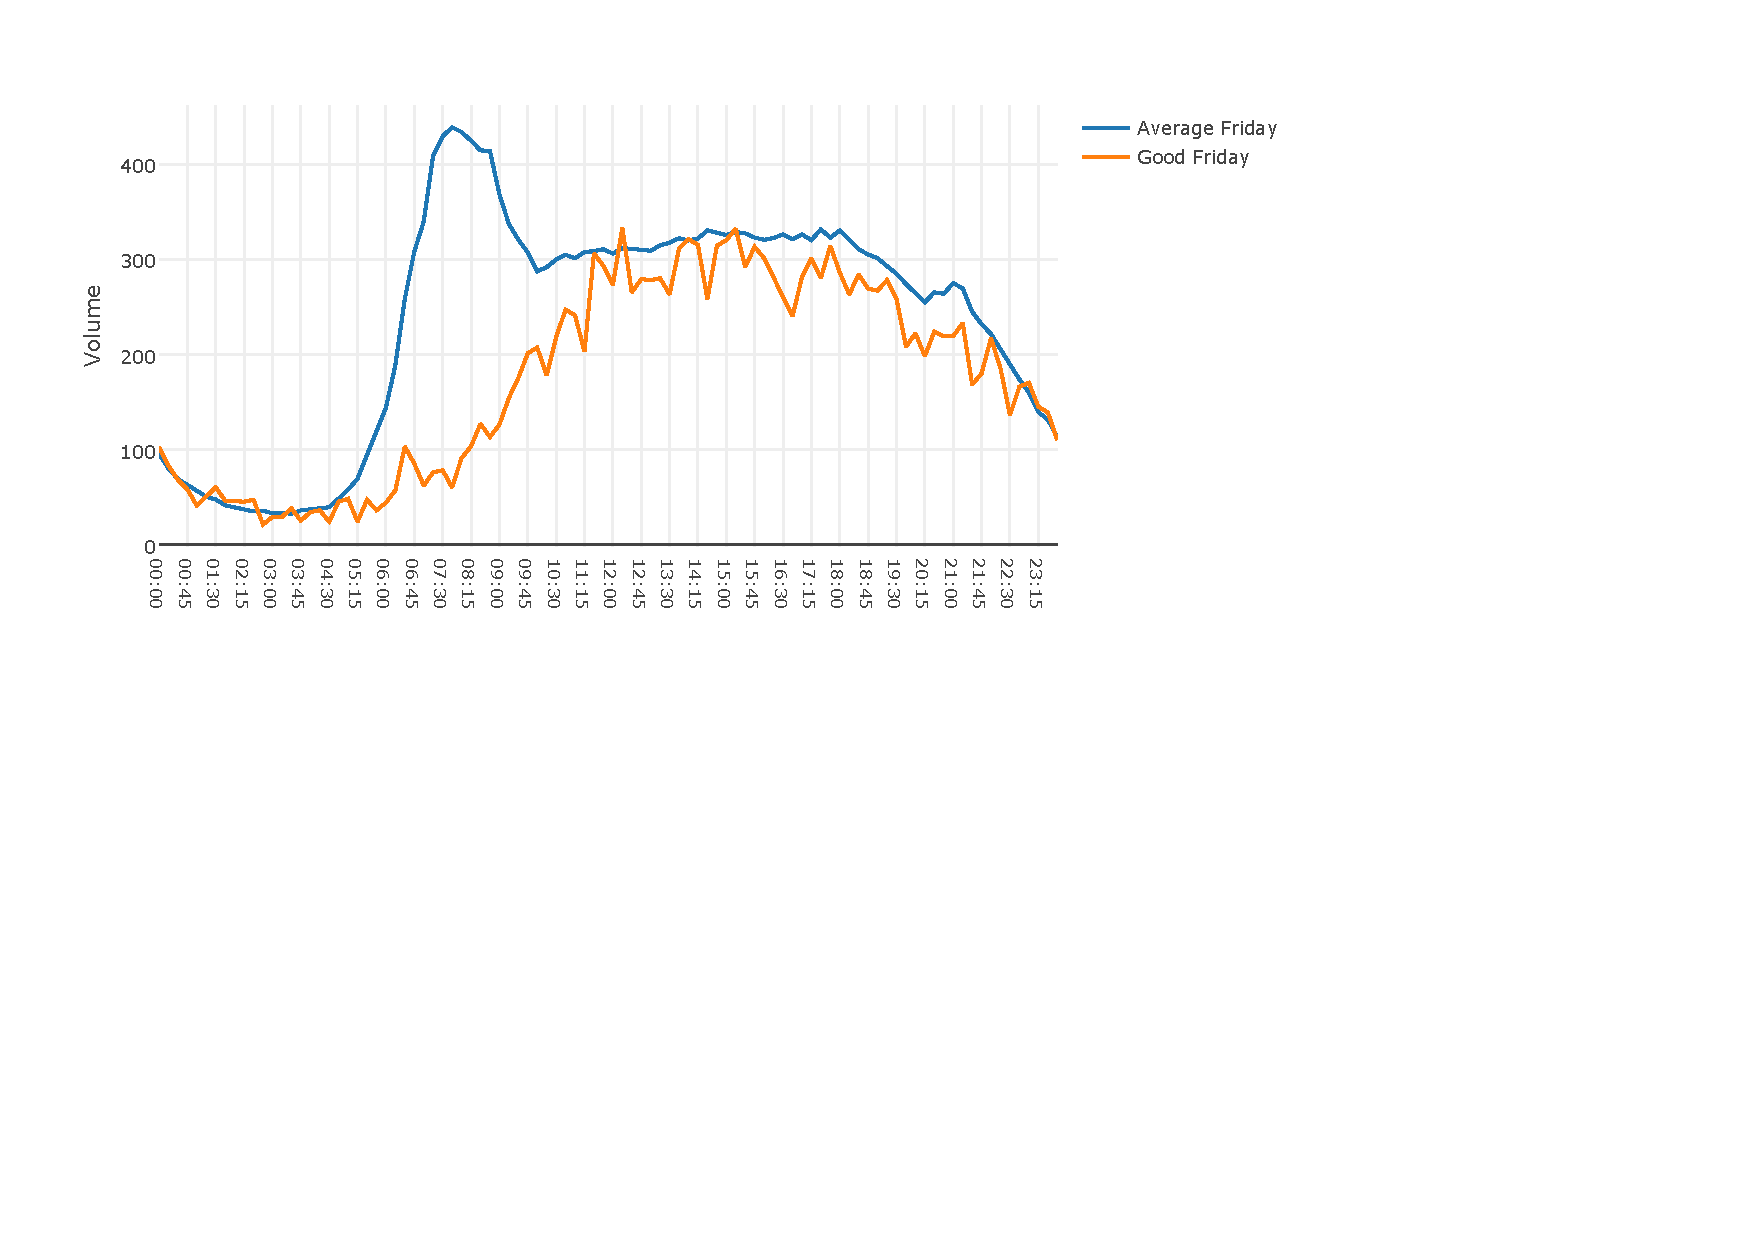
\includegraphics[width=0.4\textwidth]{Plots/holiday-fridays.pdf}
    \label{fig:HolidayFridays}}

    \caption[Impact of public holidays on traffic volume]{Variations in traffic volume caused by
     public holidays}
   \label{fig:Holidays}
\end{figure}


\subsubsection{Trends}
The secular variations in traffic volume data is important from infrastructure planning point of
view. While long term forecasting of traffic data is out of the scope for this work it is interesting
to find out the trends in the traffic volume, to see how it has evolved over the years.
Figure \ref{fig:AverageTrafficVolume} shows the average 15 minute flow on a daily, weekly,
monthly and yearly basis. From these plots We can see there is no significant trend in traffic flow.


\begin{figure}[h]
    \centering
    \subfloat[Daily][Daily]{
    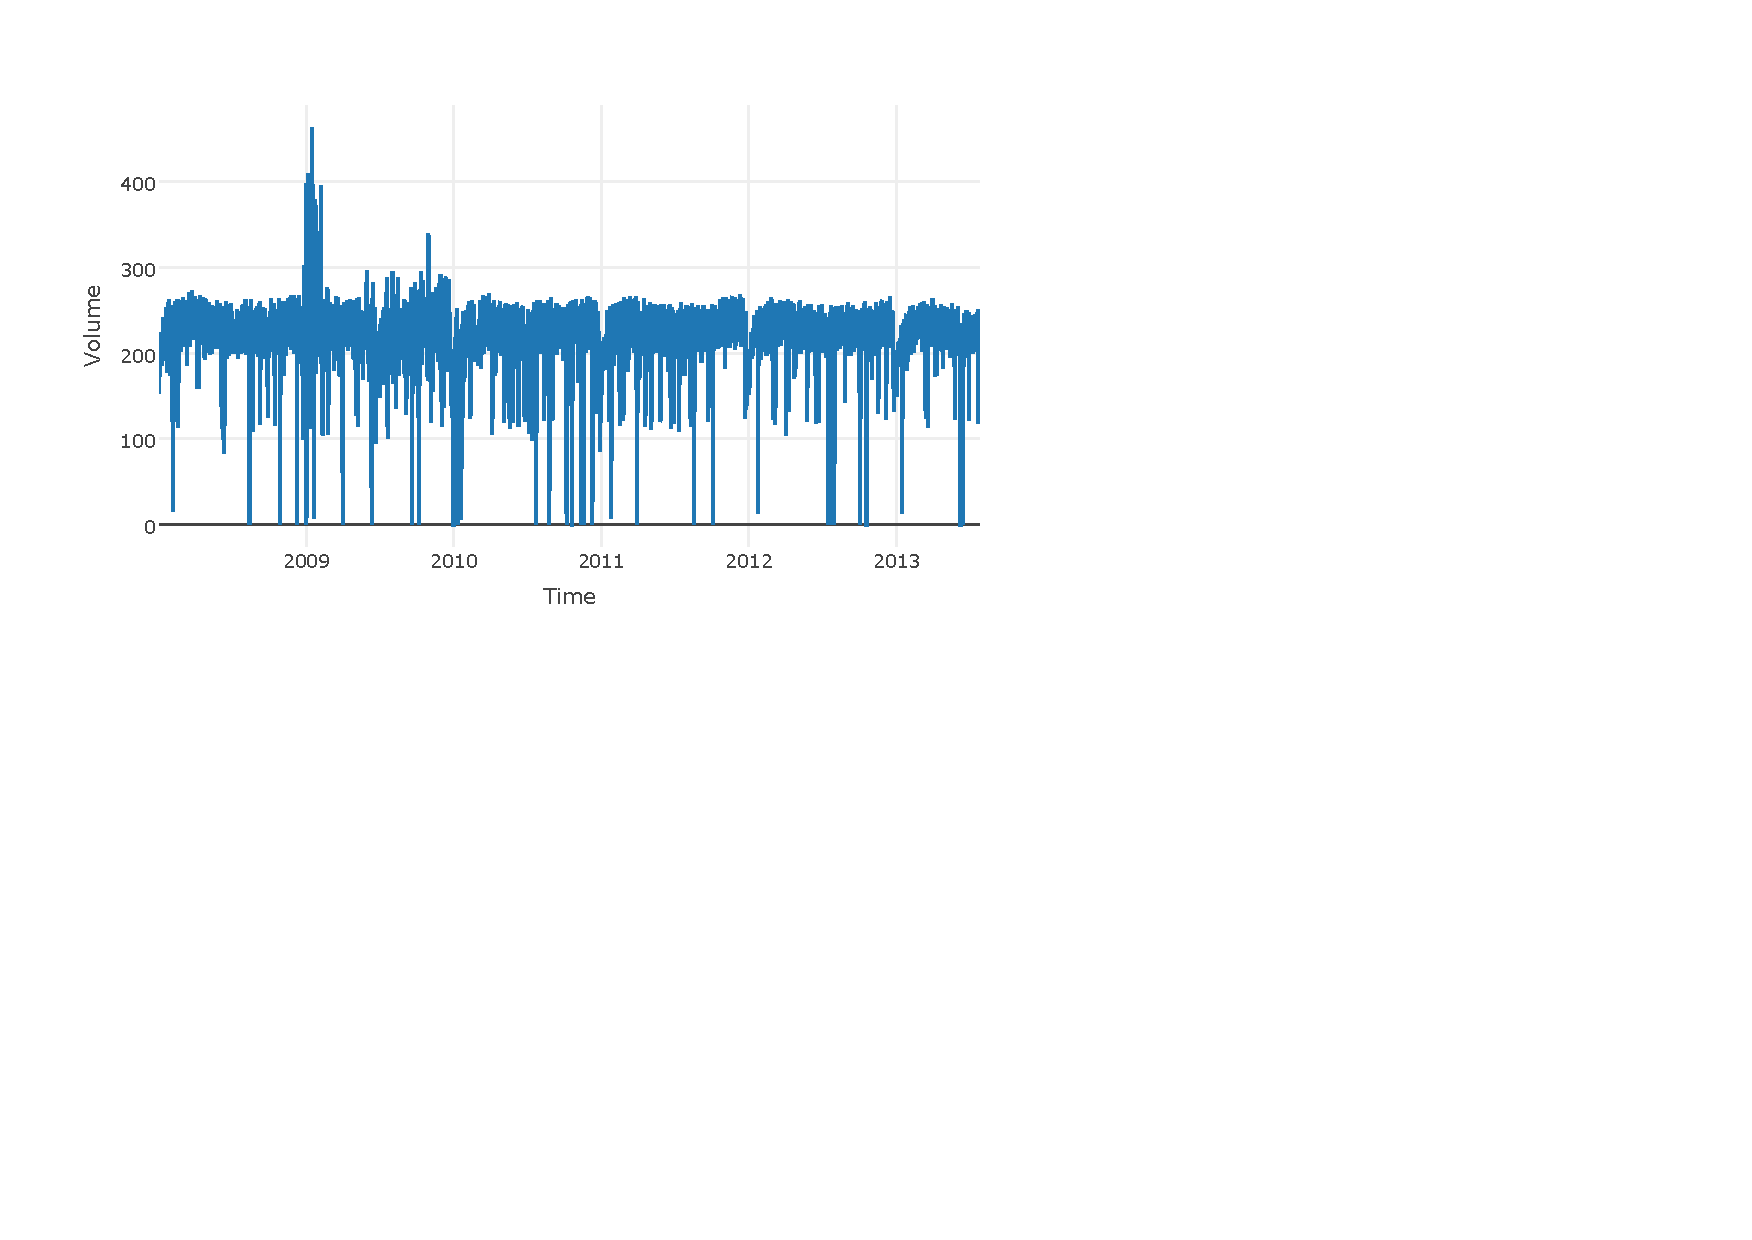
\includegraphics[width=0.4\textwidth]{Plots/averages-daily.pdf}
    \label{fig:AverageDaily}}
    \qquad
    \subfloat[Weekly][Weekly]{
    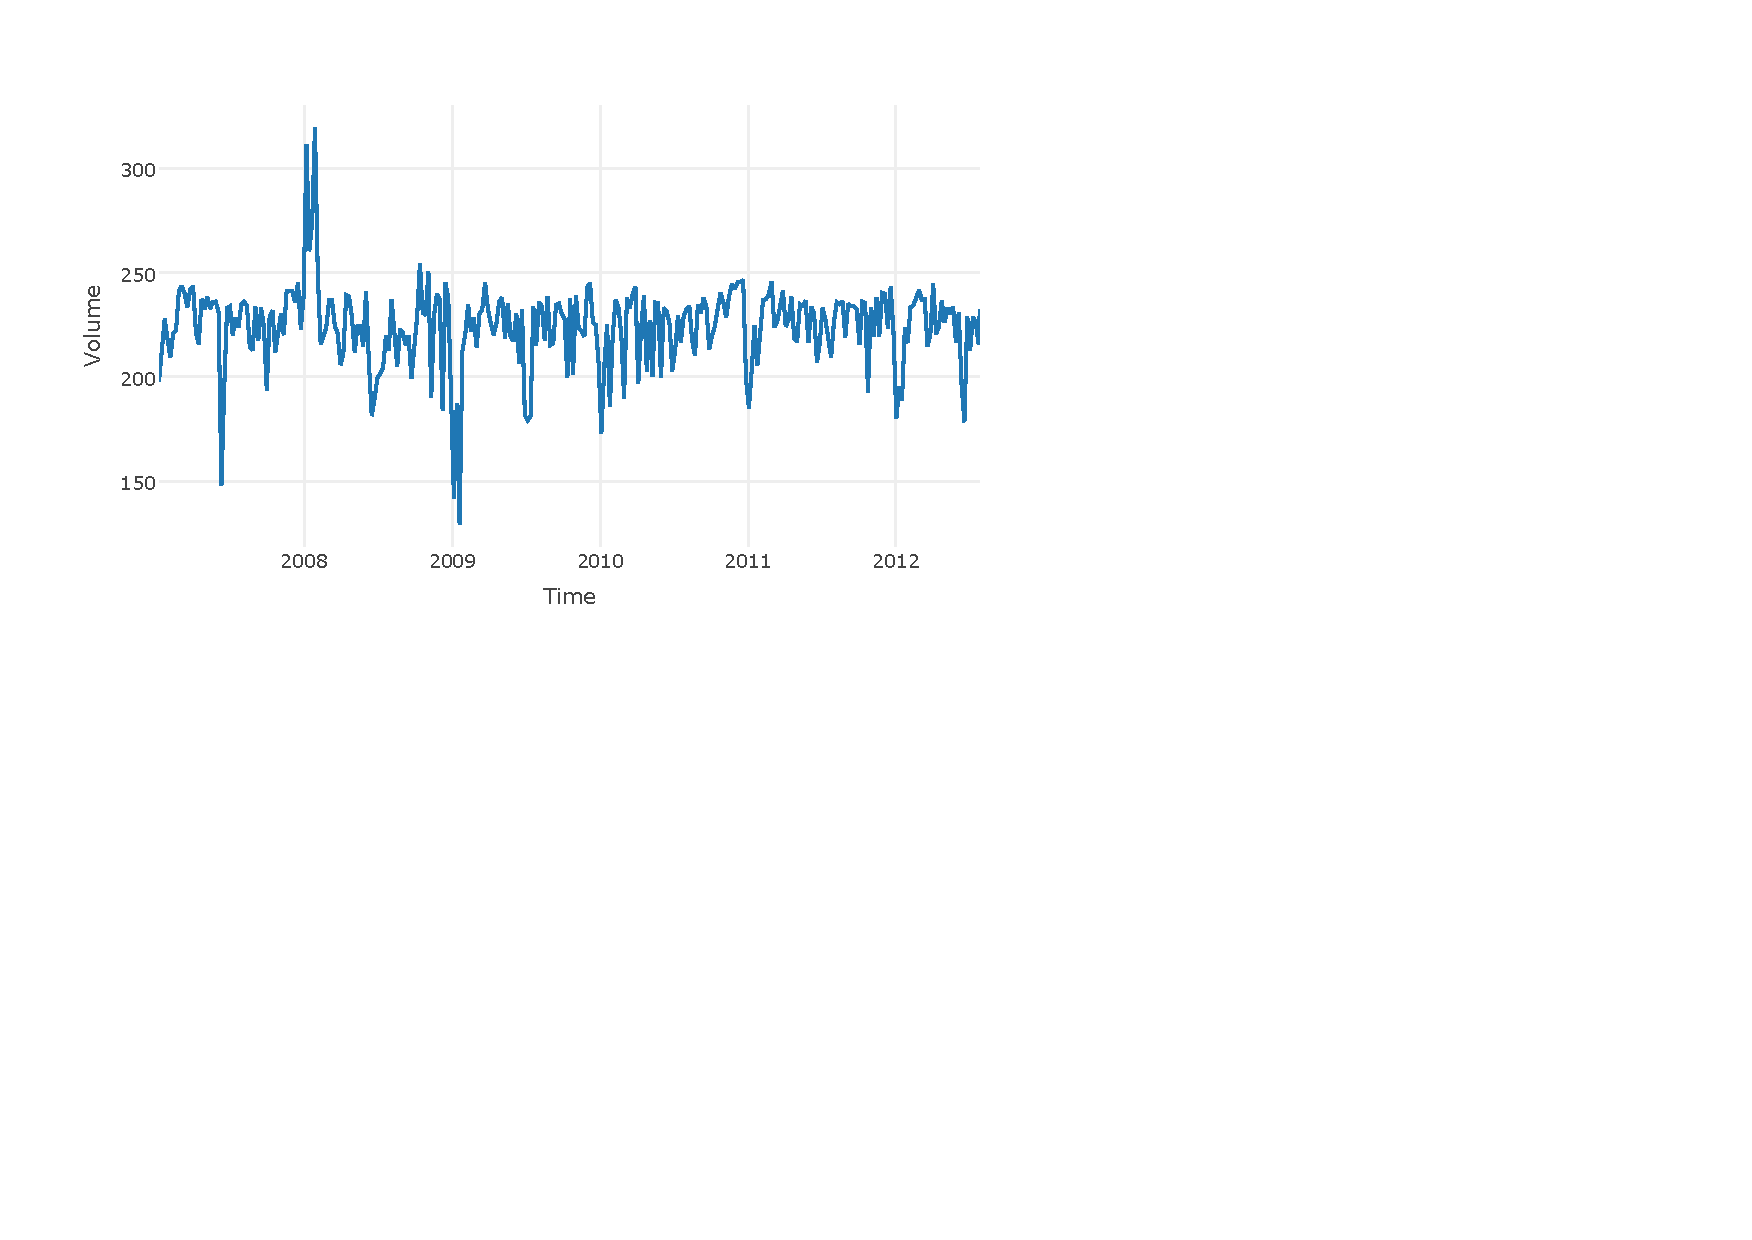
\includegraphics[width=0.4\textwidth]{Plots/averages-weekly.pdf}
    \label{fig:AverageWeekly}}

    \subfloat[Monthly][Monthly]{
    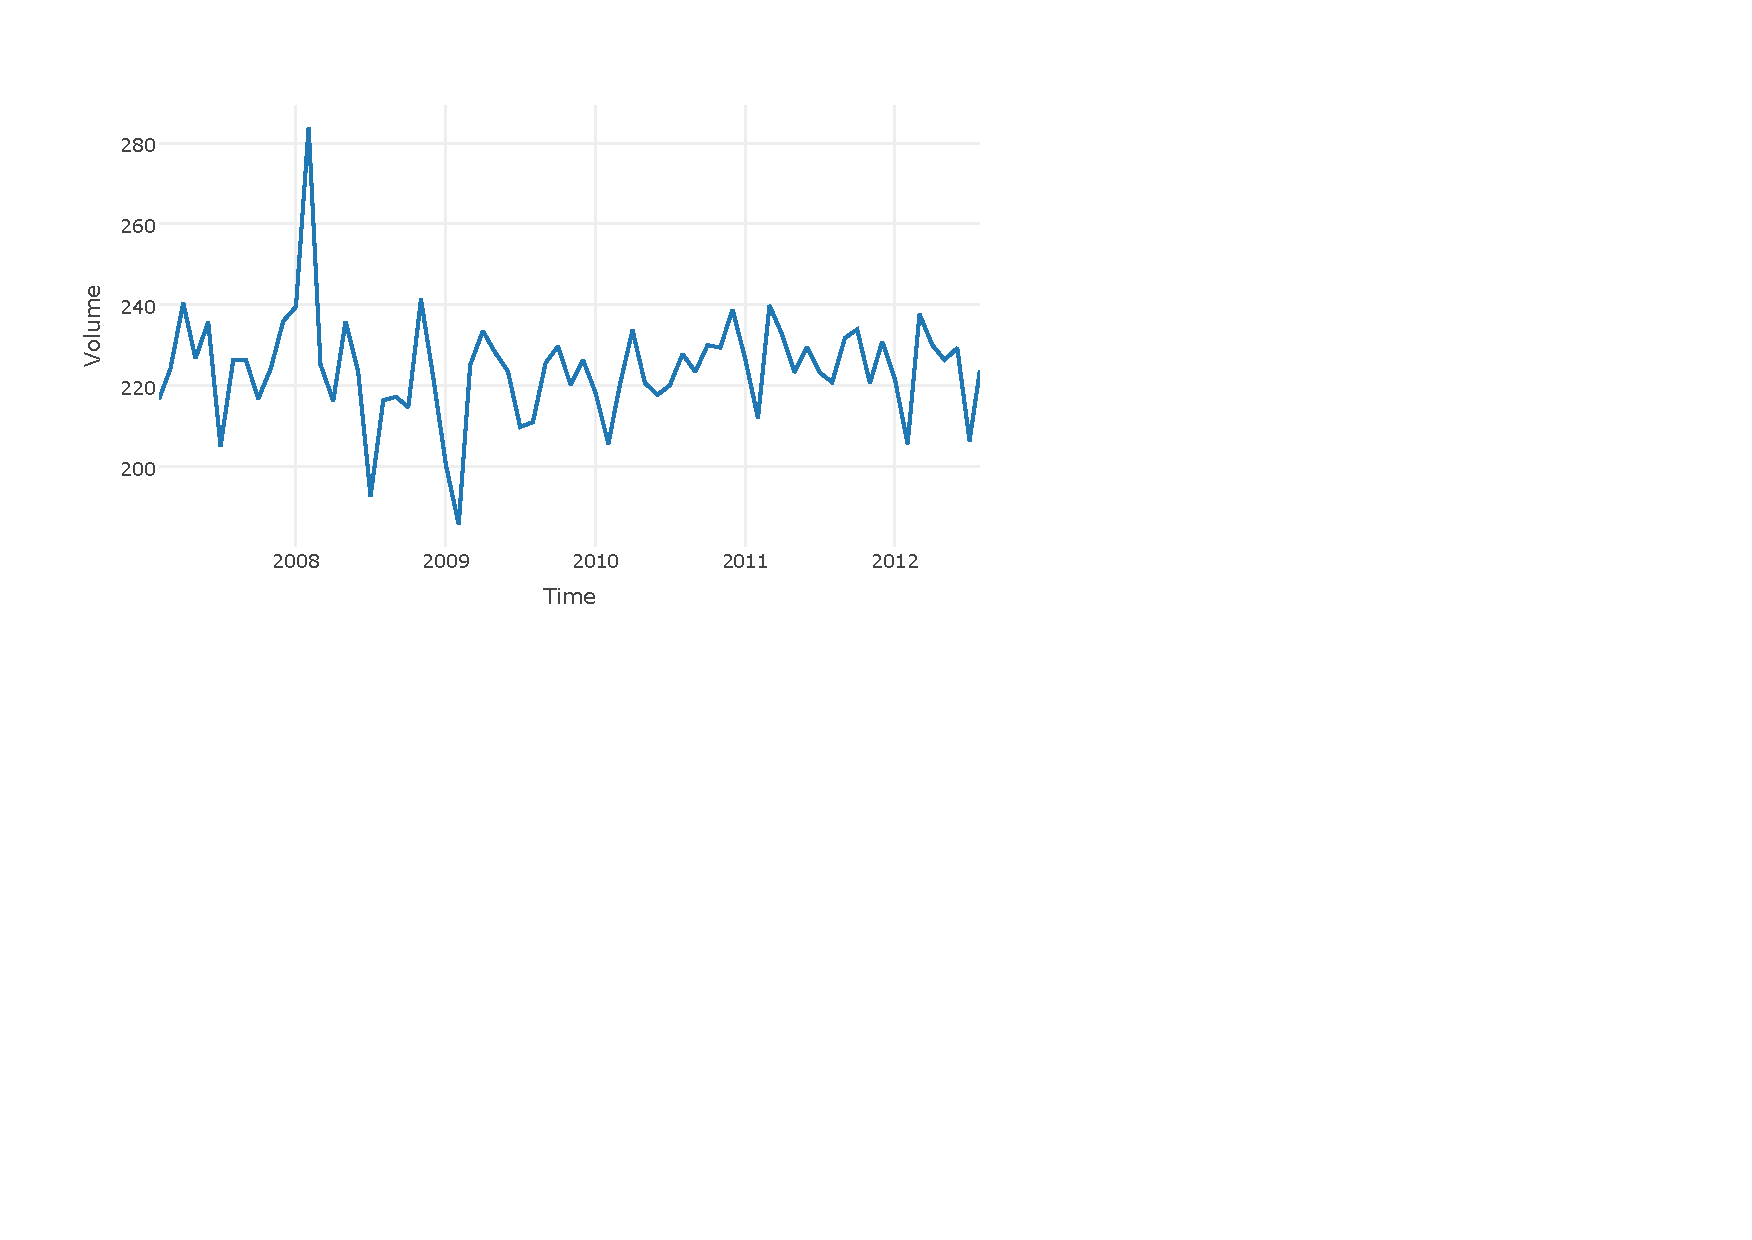
\includegraphics[width=0.4\textwidth]{Plots/averages-monthly.pdf}
    \label{fig:AverageMonthly}}
    \qquad
    \subfloat[Yearly][Yearly]{
    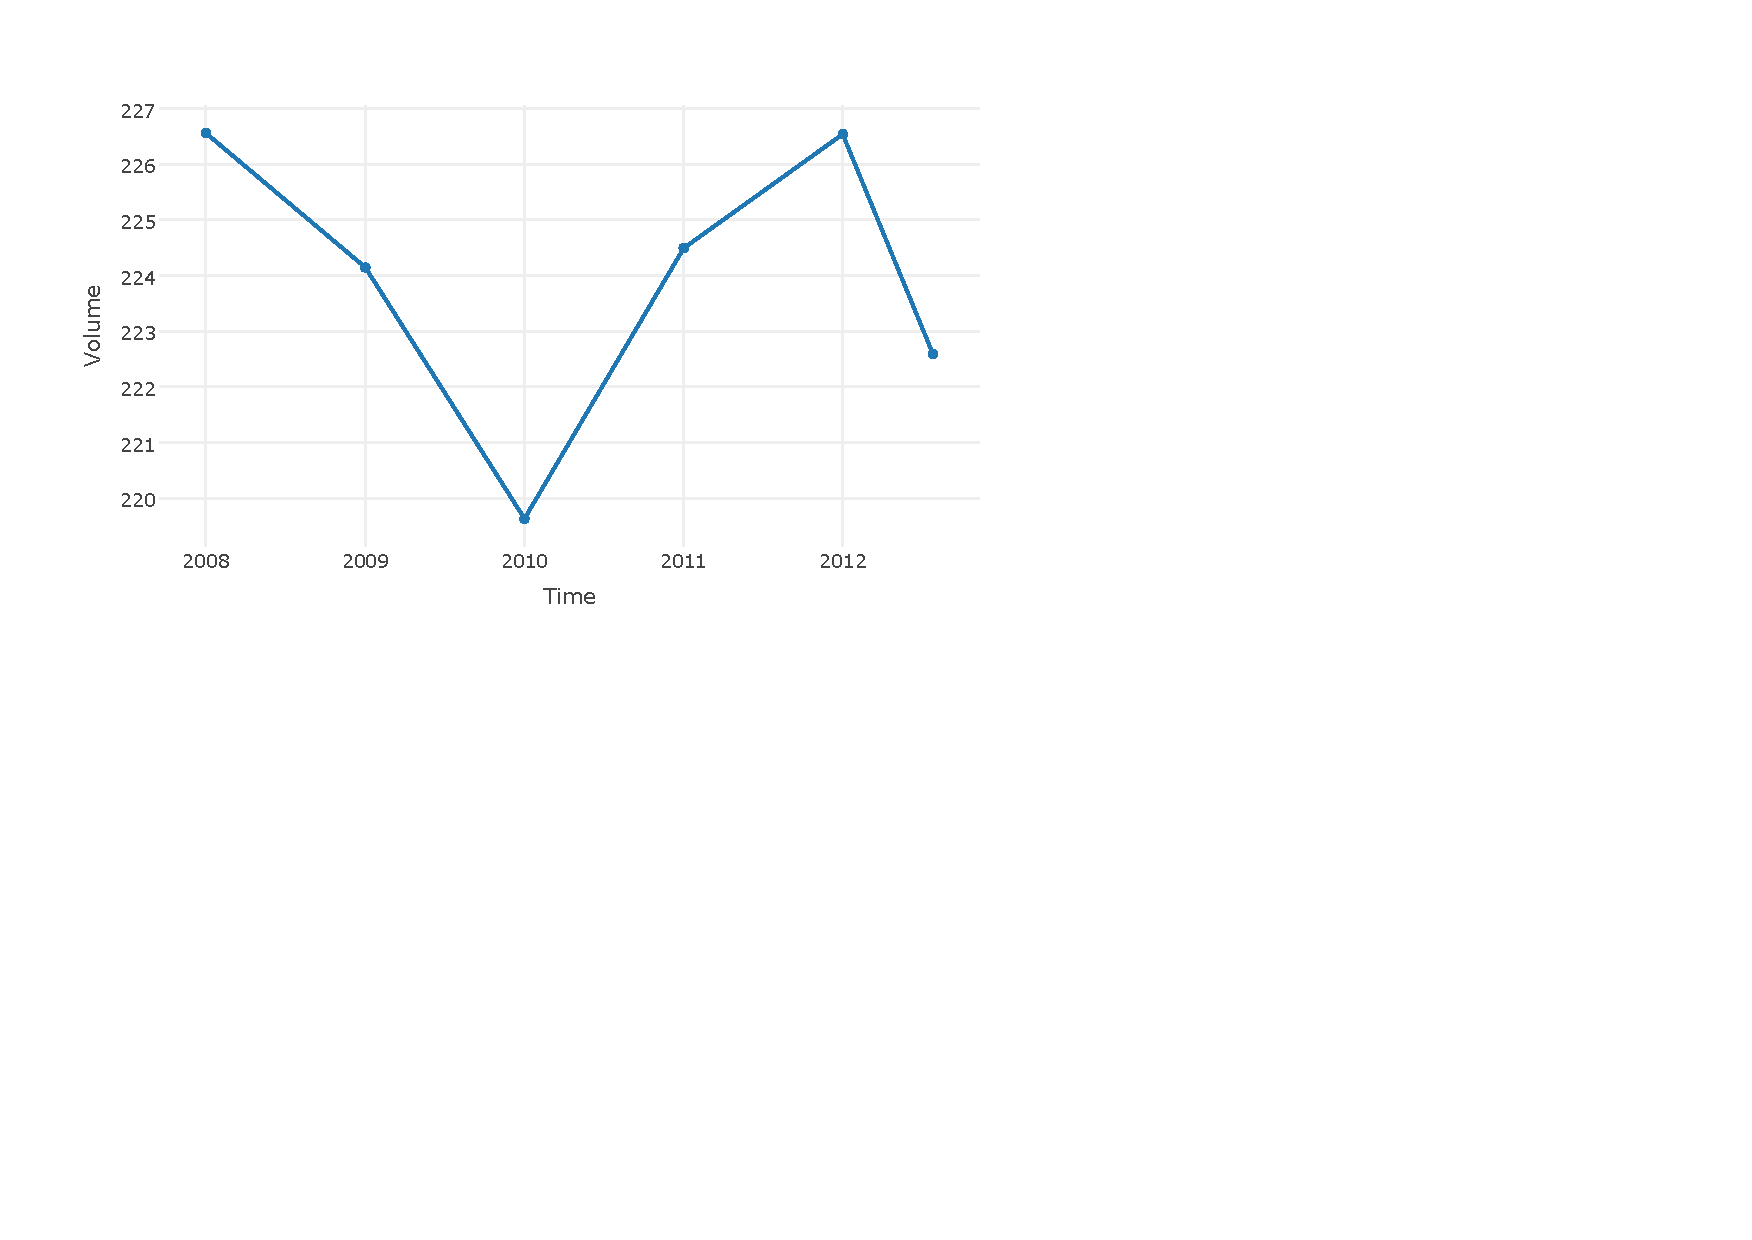
\includegraphics[width=0.4\textwidth]{Plots/averages-yearly.pdf}
    \label{fig:AverageYearly}}

    \caption[Average Traffic Volume]{(a) daily, (b) weekly, (c) monthly and (d) yearly average of
    traffic volume (15 mins interval)}
   \label{fig:AverageTrafficVolume}
\end{figure}

Moreover, we can decompose the traffic volume data, and see the different components. The plots are
shown in figure \ref{fig:trafficVolumeComponents}

\begin{figure}[h]
    \centering
    \subfloat[Time series components][Time series components]{
    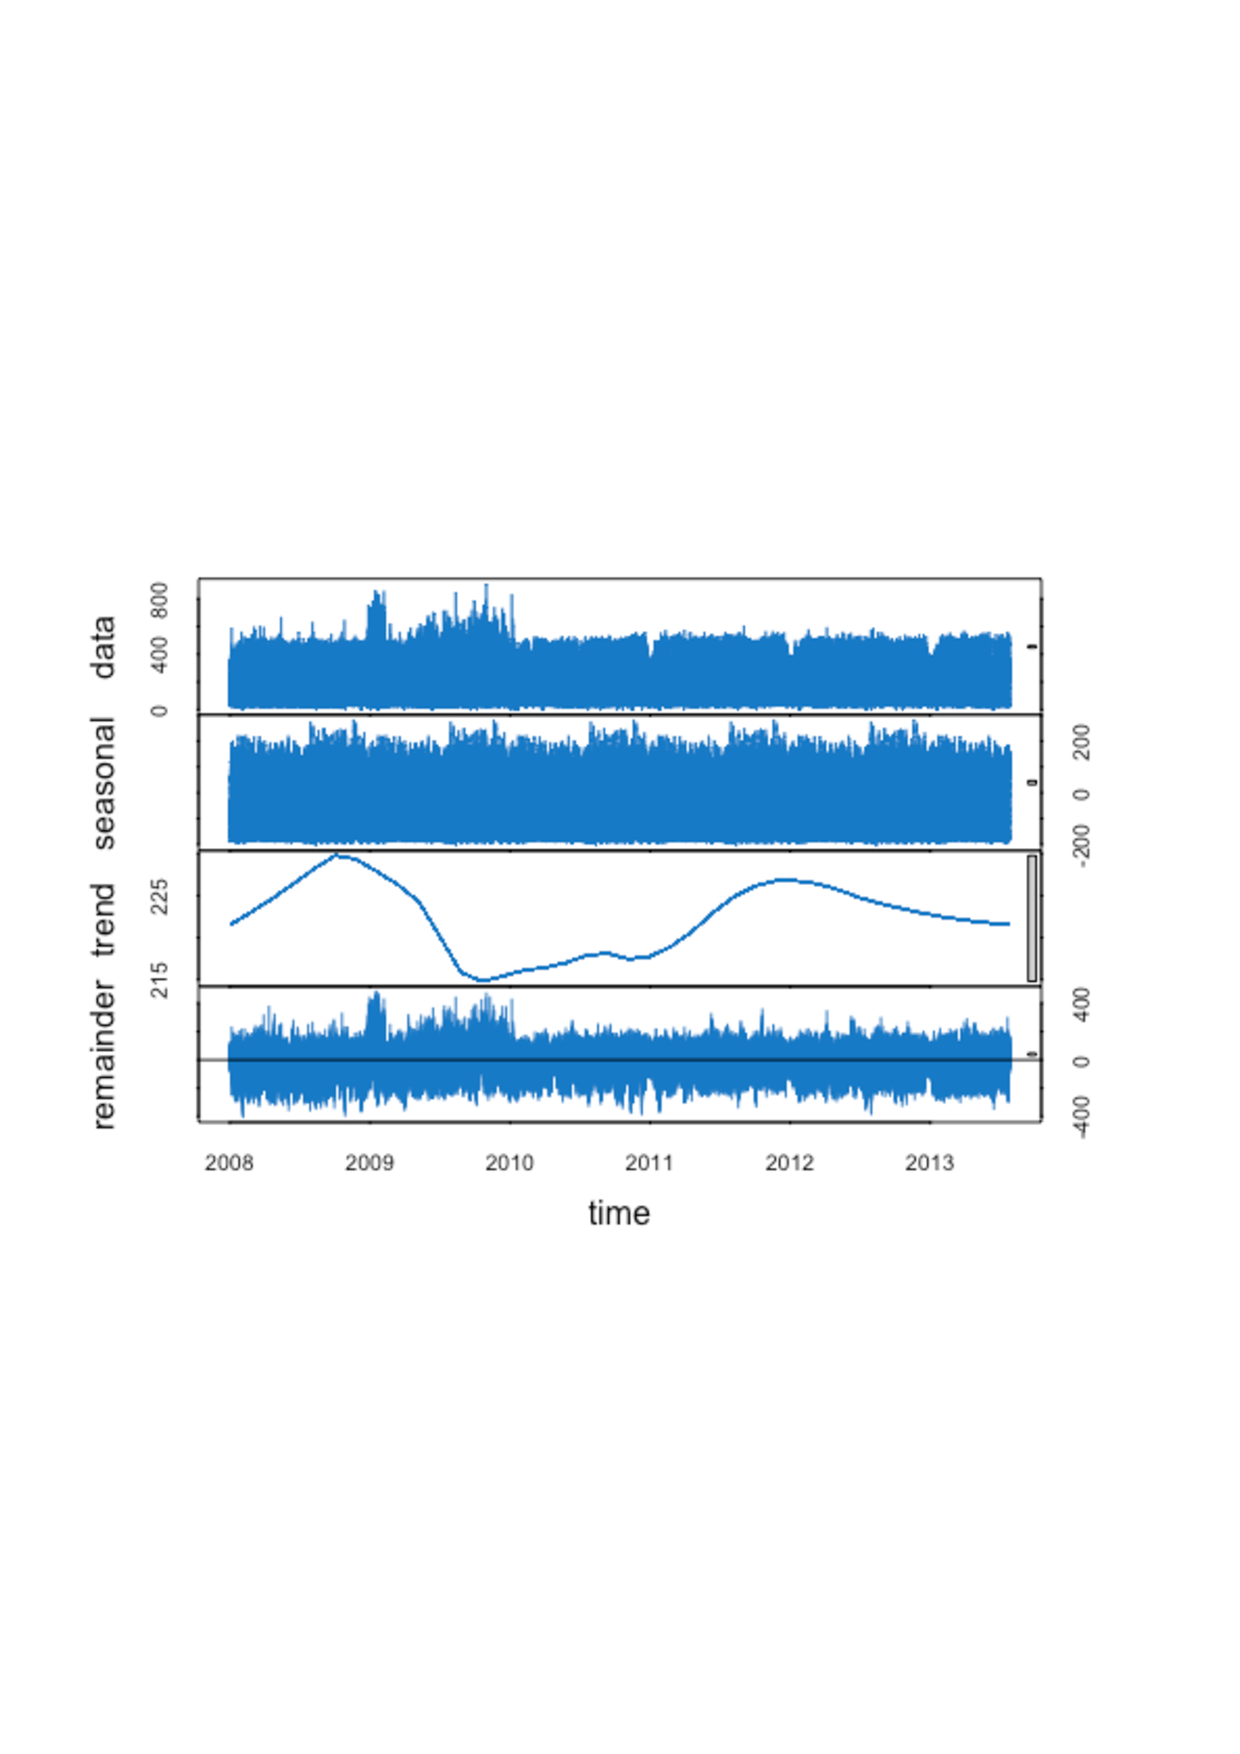
\includegraphics[width=0.4\textwidth]{Plots/decomposition.pdf}
    \label{fig:tsComponents}}
    \qquad
    \subfloat[Seasonality adjusted][Seasonality adjusted]{
    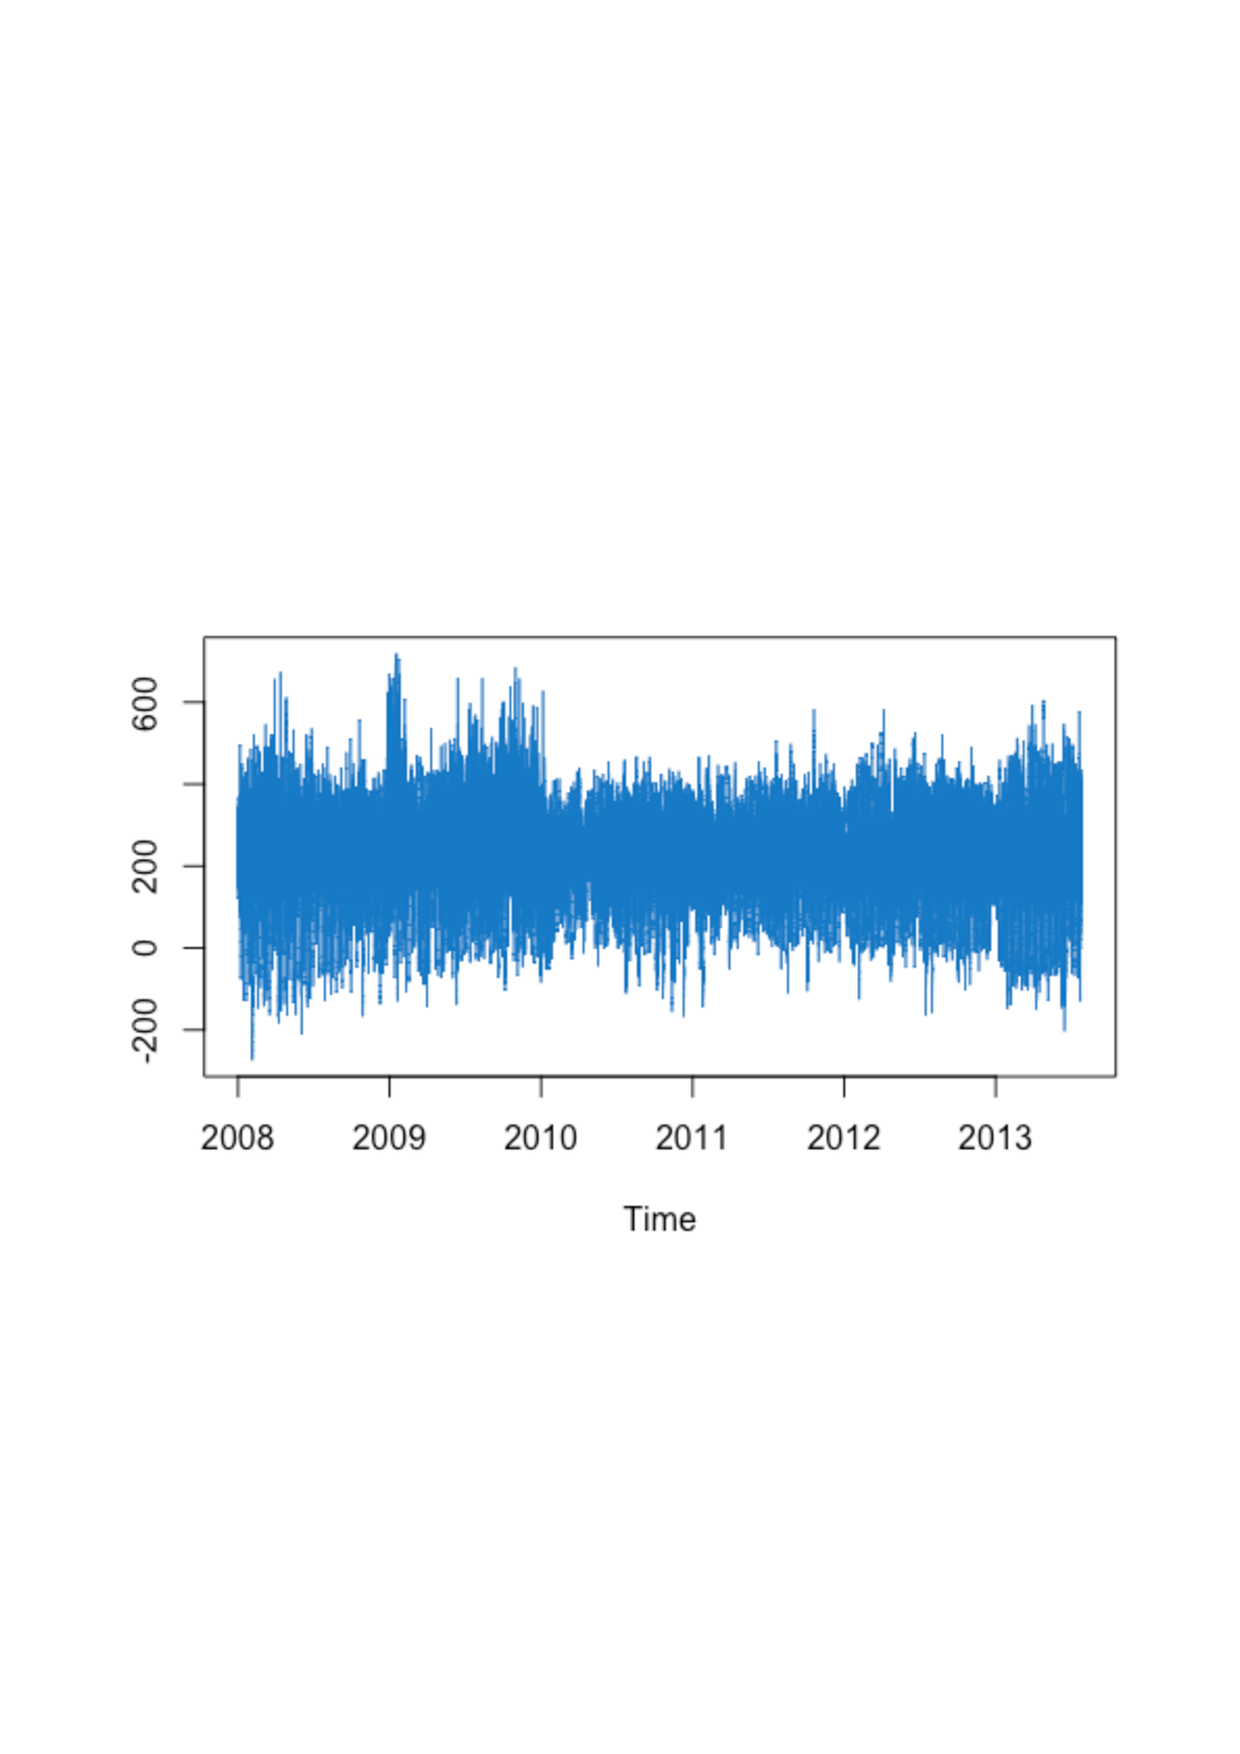
\includegraphics[width=0.4\textwidth]{Plots/season-adjusted.pdf}
    \label{fig:trafficVolumeSeasonAdj}}
    \caption[Traffic volume time series]{Traffic volume time series components and seasonality adjusted}
   \label{fig:trafficVolumeComponents}
\end{figure}



\subsection{Temporal and Spatial correlations}
We would also like to analyse the temporal relations between a series of traffic volume observations and
its own lagged values. We can see these relation by using the Auto Correlation Function (ACF) and Partial Auto
Correlation Function (PACF). The ACF gives a representation of which lag values have linear relationship
with the current observed value. The plots of these are shown in \ref{fig:trafficVolumeACFPACF}. From the
ACF, it is obvious that there is a strong correlation between the observation at time t with lags
up to 10. It means that currently observed traffic volume is shows a strong linear relationship between
past few observations.

\begin{figure}[h]
    \centering
    \subfloat[ACF][ACF]{
    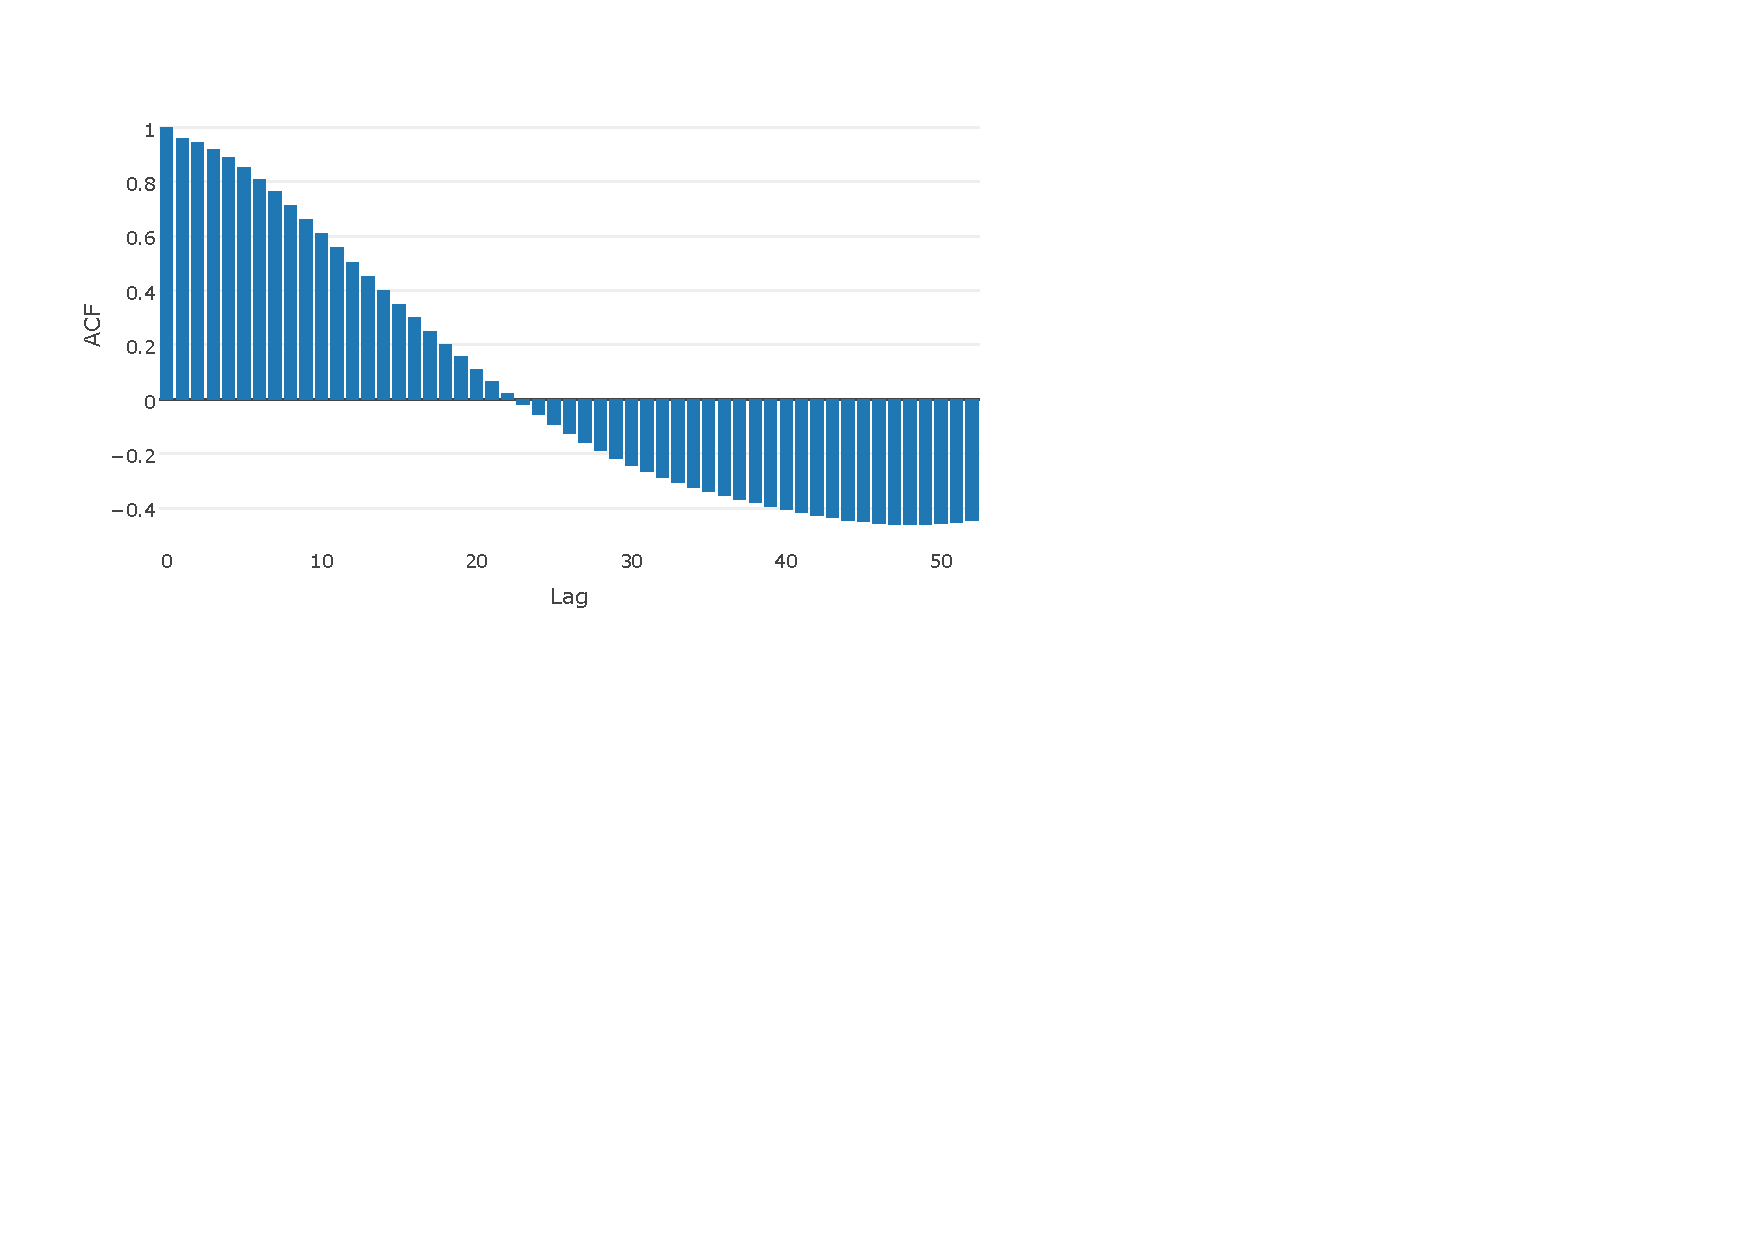
\includegraphics[width=0.4\textwidth]{Plots/acf.pdf}
    \label{fig:trafficVolumeACF}}
    \qquad
    \subfloat[PACF][PACF]{
    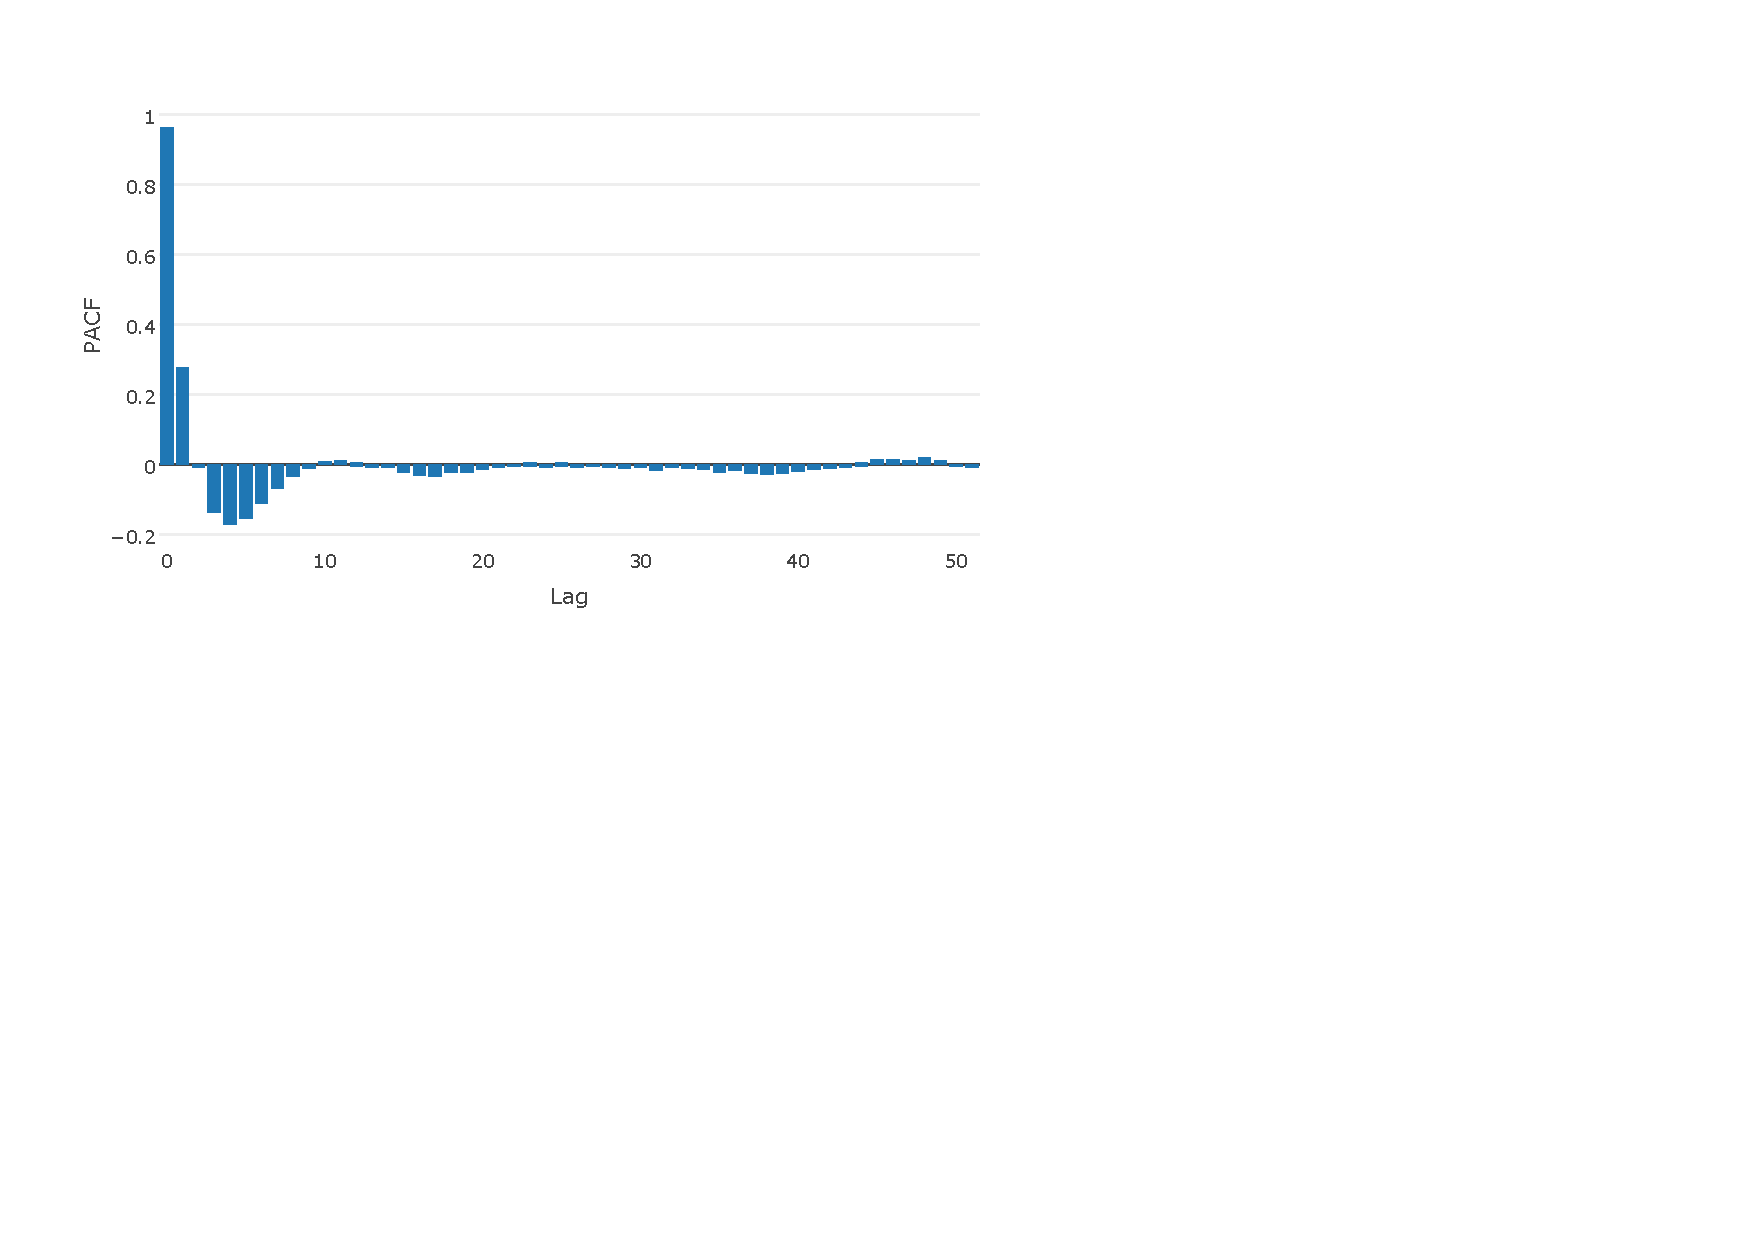
\includegraphics[width=0.4\textwidth]{Plots/pacf.pdf}
    \label{fig:trafficVolumePACF}}
    \caption[ACF and PACF]{Autocorrelation and partial autocorrelation of traffic volume time series data}
   \label{fig:trafficVolumeACFPACF}
\end{figure}

Traffic flow at upstream and adjacent locations correlate with the current location's traffic. This
spatial relations are always present in a road network and can be easily be described by the nature
of traffic movements. To analyse the spatial relations, we chose one upstream location and one
adjacent location. In figure \ref{fig:spatialCorrelation}, we show the cross correlation between the
current location's traffic volume with the upstream and adjacent location's traffic volume. We can see
that there is strong correlation between the current traffic flow with the upstream traffic flow
at lag 1, while the for correlation with the adjacent traffic flow is at lag 0.


\begin{figure}[h]
    \centering
    \subfloat[Traffic flow at upstream and adjacent locations on weekdays][Traffic flow at
    upstream and adjacent locations on weekdays]{
    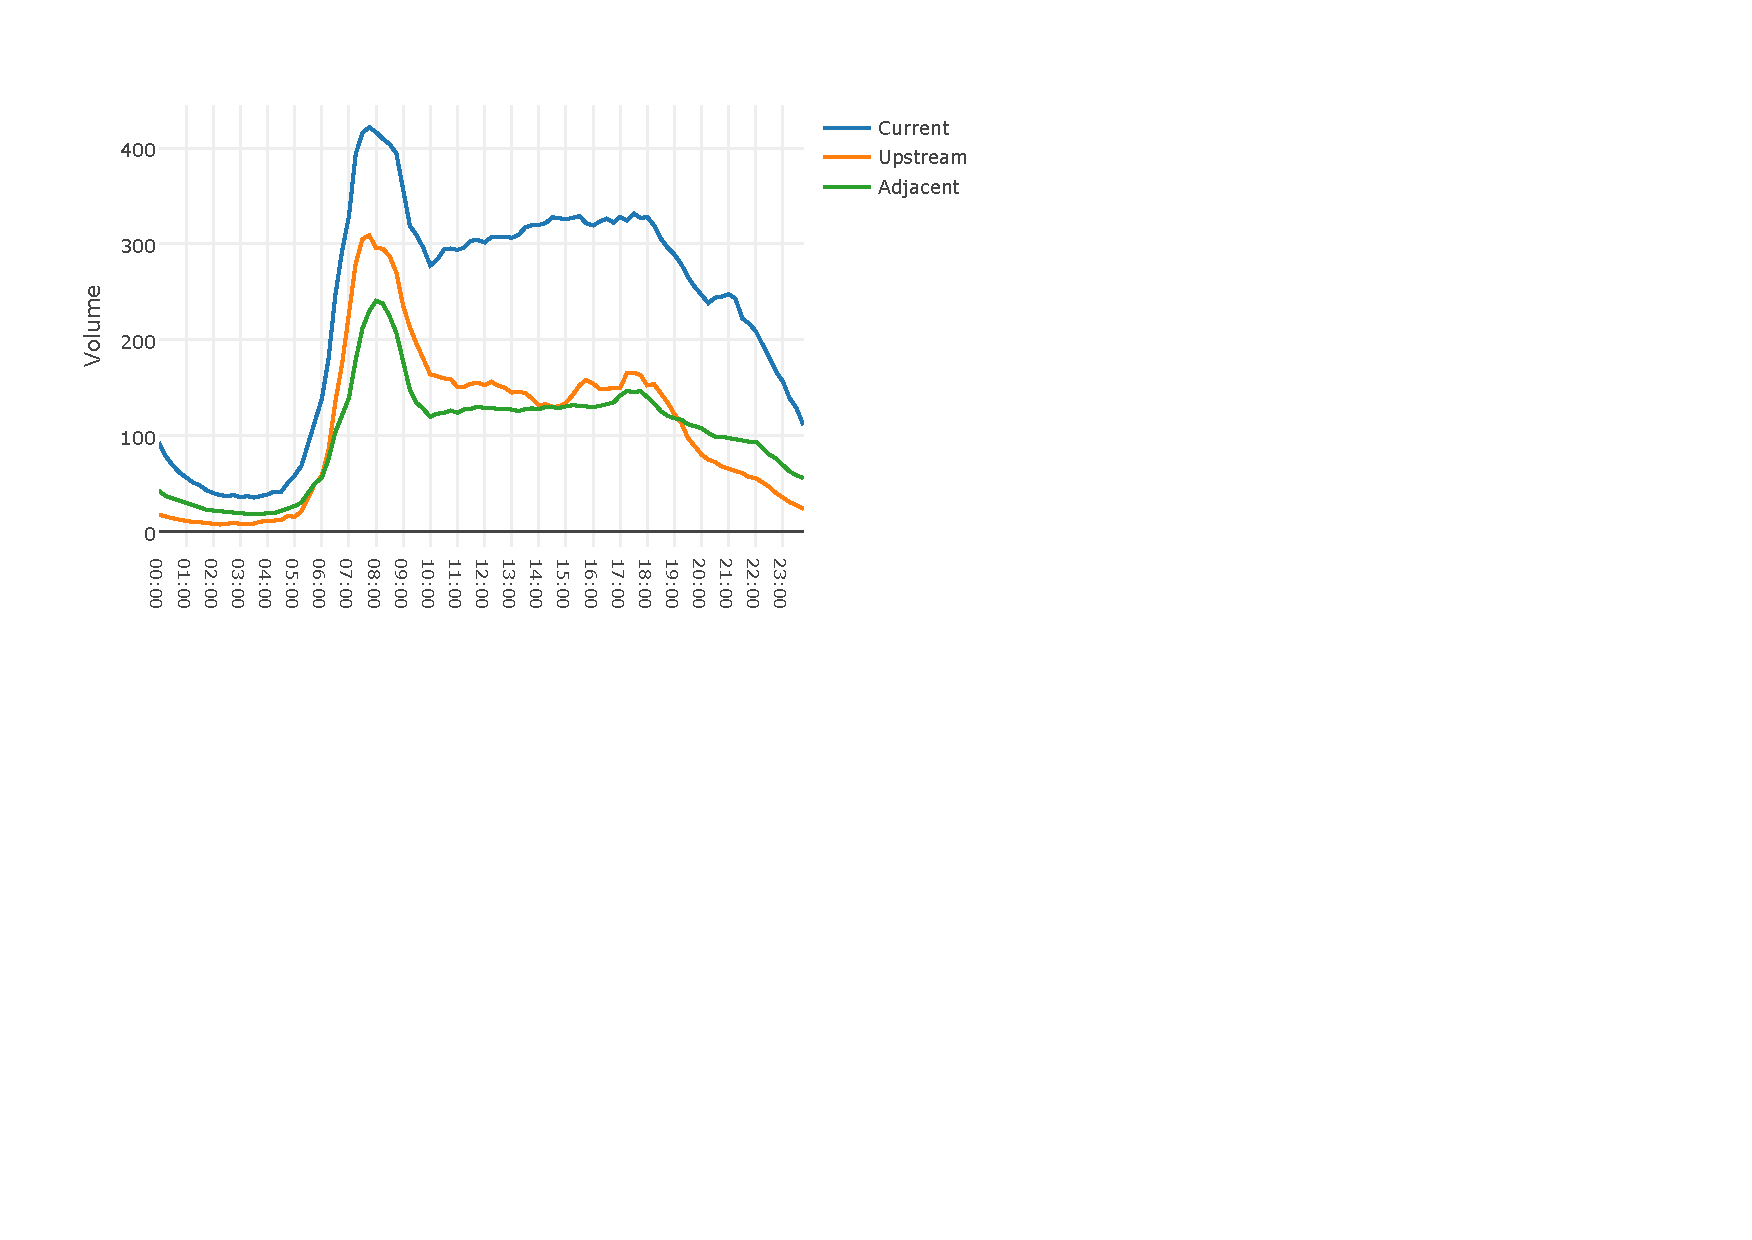
\includegraphics[width=0.4\textwidth]{Plots/spatial-weekdays.pdf}
    \label{fig:spatialWeekdays}}
    \qquad
    \subfloat[Traffic flow at upstream and adjacent locations on weekends][Traffic flow at upstream
    and adjacent locations on weekdays]{
    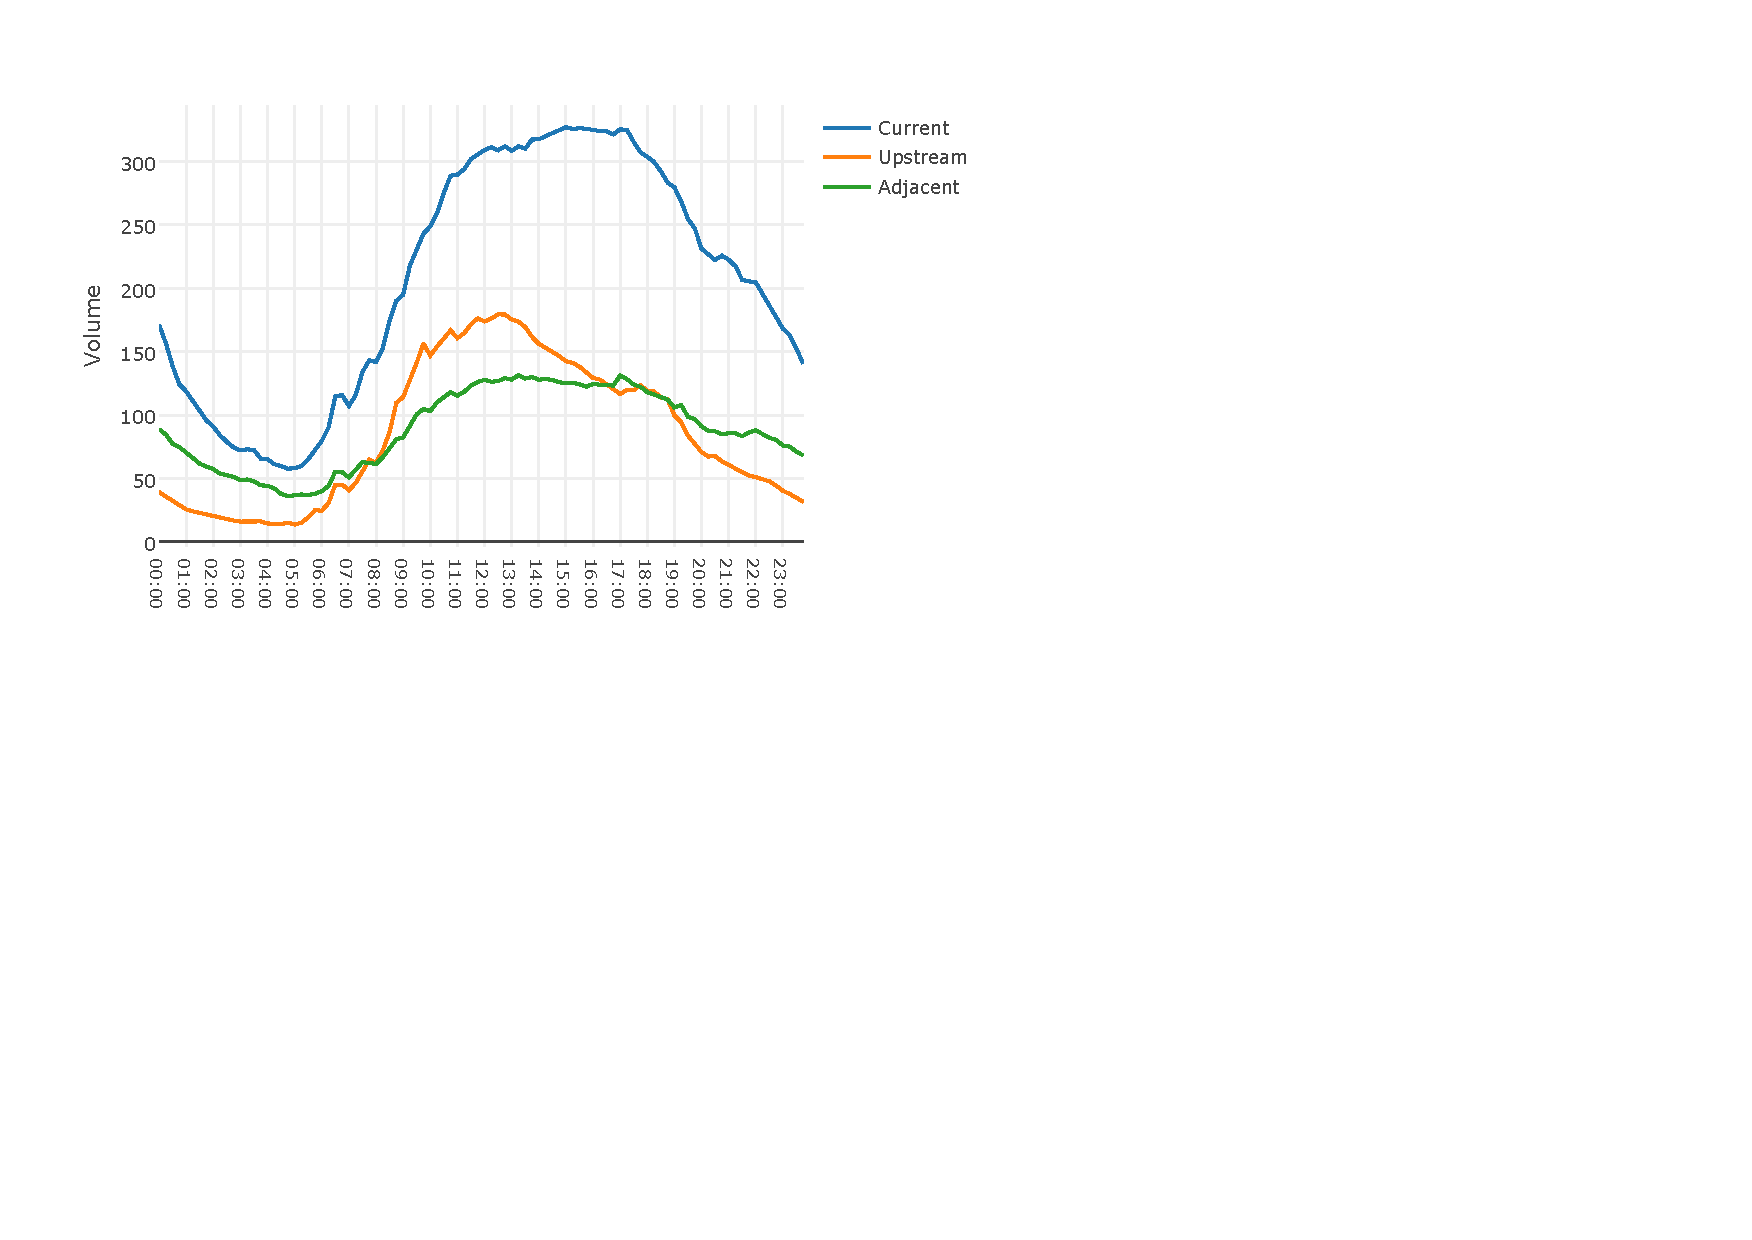
\includegraphics[width=0.4\textwidth]{Plots/spatial-weekends.pdf}
    \label{fig:spatialWeekends}}

    \subfloat[Upstream traffic][Upstream traffic]{
    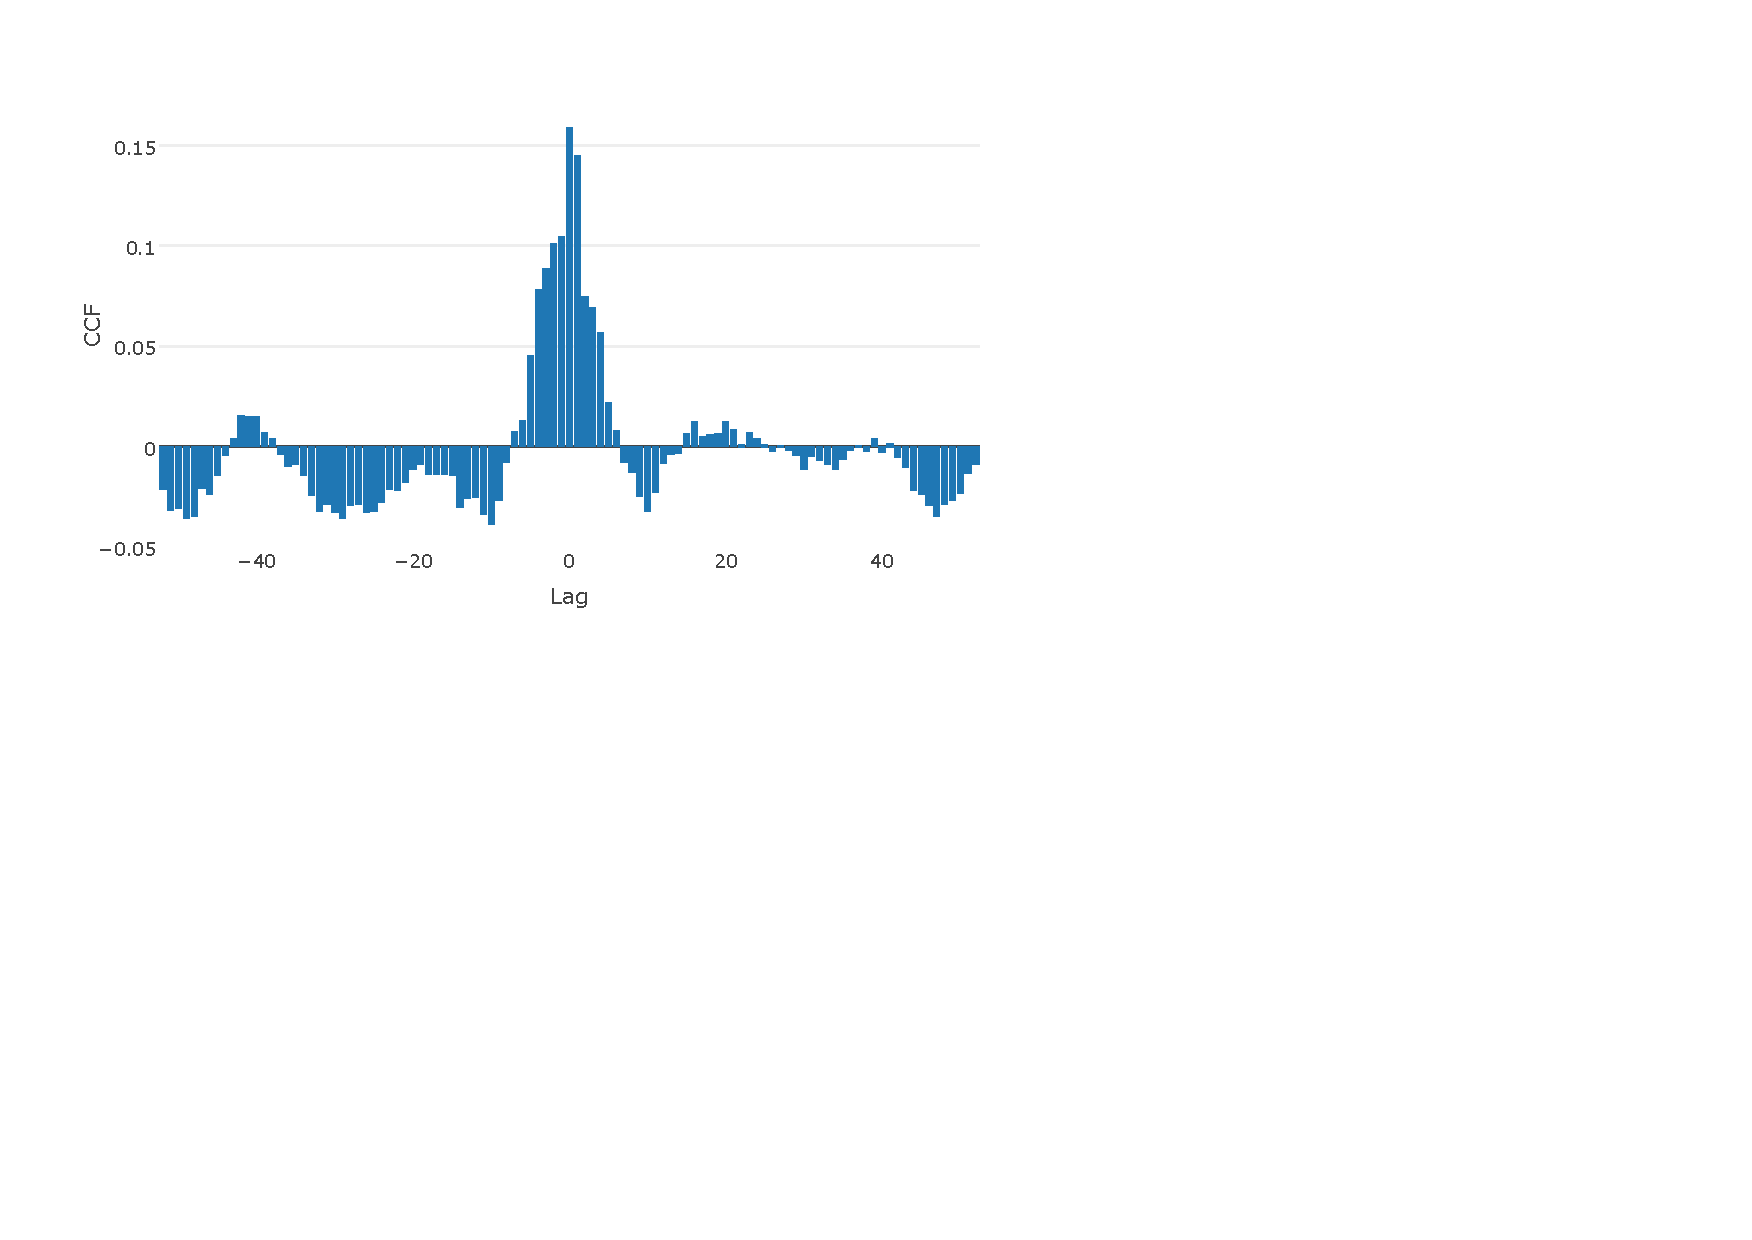
\includegraphics[width=0.4\textwidth]{Plots/ccf1.pdf}
    \label{fig:upstreamTraffic}}
    \qquad
    \subfloat[Adjacent traffic][Adjacent traffic]{
    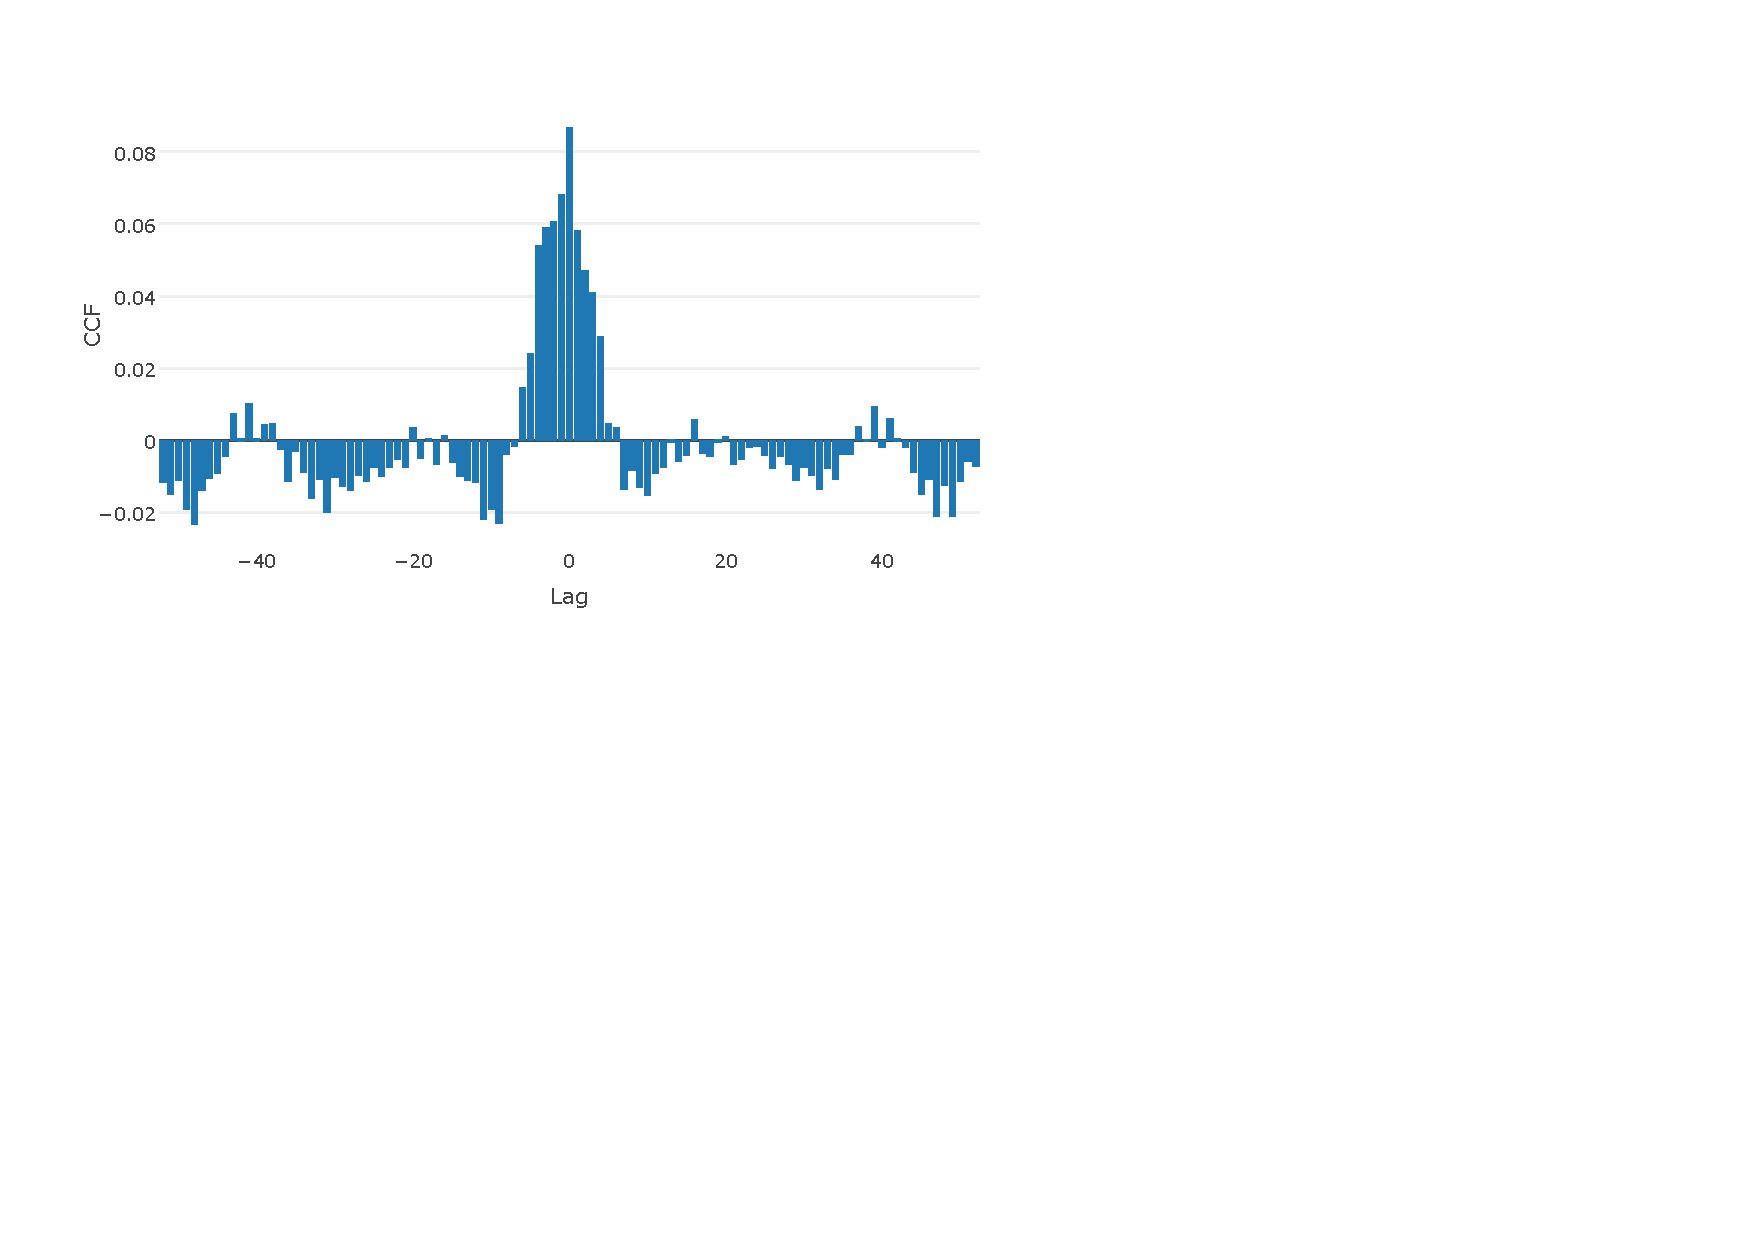
\includegraphics[width=0.4\textwidth]{Plots/ccf2.pdf}
    \label{fig:adjacentTraffic}}
    \caption[Spatial correlations between traffic volume]{Spatial correlations between traffic volume
    data from different locations. (a) and (b) shows the average traffic flow on weekdays and weekends
    at the current, upstream and adjacent locations. Figure (c) and (d) shows the plots of cross-correlation
    functions between the current location and upstream and adjacent location.}
   \label{fig:spatialCorrelation}
\end{figure}